%\documentclass[preprint,10pt]{elsarticle}
\documentclass{jfm}

%\usepackage{algorithmic}
%\usepackage{algorithm}
\usepackage{amsfonts}
\usepackage[fleqn,reqno]{amsmath}
\usepackage{amssymb}
%\usepackage{amsthm}
\usepackage[titletoc]{appendix}
\usepackage{array}
%\usepackage{bm}
%\usepackage{caption}
%\usepackage[usenames]{color}
\usepackage{enumitem}
%\usepackage{epsfig}
%\usepackage{fancybox}
\usepackage{filecontents}
\usepackage[top=1.2in,bottom=1.2in,left=1in, right=1in]{geometry}
\usepackage{graphics}
%%\usepackage{ifthen}
\usepackage{lineno}
%\usepackage{mathrsfs}
%\usepackage{mdframed}
%\usepackage{multirow}
%\usepackage{palatino}
%\usepackage{showkeys} %To see the labels for now.  Will remove later
%\usepackage{stmaryrd}
%\usepackage{subfigure}
%\usepackage{paralist}
\usepackage{pgfplots}
%\usepackage{tabularx}
\usepackage{tikz}
\usepackage{todonotes}
\usetikzlibrary{arrows}
\usepackage{comment}

%%%%%%  pdftex  %%%%%%%%%%%%%%%%%%%%%%%%%%%%%%%%%%%%%%%%%%%%%%%%%%%%%%
\usepackage[pagebackref=false,bookmarks=false]{hyperref} 

\hypersetup{
  bookmarksnumbered=true,
  bookmarksopen=false,
  hypertexnames=false,      
  breaklinks=true,          
  unicode=false,
  pdffitwindow=true,        
  pdfnewwindow=true,        
  colorlinks=true,         
  linkcolor=dblue,
  anchorcolor=red,
  citecolor=dorange,
  filecolor=magenta,
  urlcolor=dblue,
  pdfstartview = FitH,
  pdfkeywords = {},
  pdfcreator = {LaTeX with hyperref package}
}



\newcommand{\bd}{{\partial}}
\newcommand{\bigO}{{\mathcal{O}}}
\newcommand{\cc}{{\mathbf{c}}}
\newcommand{\DD}{{\mathcal{D}}}
\newcommand{\eeta}{{\boldsymbol\eta}}
\newcommand{\ff}{{\mathbf{f}}}
\newcommand{\grad}{{\nabla}}
\newcommand{\II}{{\mathbf{I}}}
\newcommand{\iin}{\mathrm{in}}
\newcommand{\llambda}{{\boldsymbol\lambda}}
\newcommand{\nn}{{\mathbf{n}}}
\newcommand{\NN}{{\mathcal{N}}}
\newcommand{\out}{\mathrm{out}}
\newcommand{\rr}{{\mathbf{r}}}
\newcommand{\RR}{{\mathbb{R}}}
\renewcommand{\ss}{{\mathbf{s}}}
\newcommand{\ssigma}{{\boldsymbol\sigma}}
\newcommand{\tar}{\mathrm{tar}}
\newcommand{\uu}{{\mathbf{u}}}
\newcommand{\UU}{{\mathbf{U}}}
\newcommand{\vv}{{\mathbf{v}}}
\newcommand{\xx}{{\mathbf{x}}}
\newcommand{\xxi}{{\boldsymbol{\xi}}}
\newcommand{\yy}{{\mathbf{y}}}

\def\gap{\hspace*{.2in}}

% Derivatives
\newcommand{\pderiv}[2]{\frac{\partial #1}{\partial #2}}
\newcommand{\tderiv}[2]{\frac{d #1}{d #2}}
\newcommand{\ppd}[2]{\frac{\partial^2 #1}{{\partial #2}^2}}

% Nick's commands
\newcommand{\vsp}[1]{\vspace{#1 pc} \noindent}
\newcommand{\abs}[1]{\lvert #1 \rvert}
\newcommand{\mean}[1]{\left< #1 \right>}
\newcommand{\thL}{$\theta$--$L$}
\newcommand{\eps}{\varepsilon}
\newcommand{\Vn}{V_n}
\newcommand{\Vs}{V_s}
\newcommand{\atau}{\abs{\tau}}
\newcommand{\thalpha}{\pderiv{\theta}{\alpha}}
\newcommand{\elfun}{\zeta}
\newcommand{\thhat}{\hat{\theta}}
\newcommand{\Dt}{\Delta t}
\newcommand{\NLterm}{\mathcal{N}}
\newcommand{\Mterm}{\mathcal{M}}
\newcommand{\FourierSum}{ \sum_{k = -N_\iin /2}^{N_\iin /2-1} }
\newcommand{\atausig}{\atau^{(\sigma)}}
\newcommand{\Vnsig}{\Vn^{(\sigma)}}
\newcommand{\Vssig}{\Vs^{(\sigma)}}


\newcommand{\tauD}[1]{\tau_{#1\text{D}}}
\newcommand{\atauD}[1]{\abs{\tau_{#1\text{D}}}}

%\usepackage{showkeys}

\shorttitle{Viscous Transport in Eroding Porous Media}
\shortauthor{Chiu, Moore and Quaife}

\title{Viscous Transport in Eroding Porous Media}

\author{Shang-Huan Chiu\aff{1}, M.~N.~J.~Moore\aff{2}, and Bryan
Quaife\aff{3}\corresp{\email{bquaife@fsu.edu}}}
  
%  Alan N. Other\aff{1}
%  \corresp{\email{jfm@damtp.cam.ac.uk}},
%  H. - C. Smith\aff{1}
% \and J. Q.  Public\aff{2}}

\affiliation{
\aff{1}Department of Scientific Computing, Florida State University,
Florida State University, Tallahassee, FL 32306, USA
\aff{2}Department of Mathematics and Geophysical Fluid Dynamics
Institute, Florida State University, Tallahassee, FL 32306, USA
\aff{3}Department of Scientific Computing and Geophysical Fluid Dynamics
Institute, Florida State University, Tallahassee, FL 32306, USA
}

\begin{document}

\maketitle

%\title{Viscous Transport in Eroding Porous Media}
%
%\author[SH]{Shang-Huan Chiu}
%\author[Nick]{M.~N.~J.~Moore}
%\author[Bryan]{Bryan D.~Quaife}
%
%\address[SH]{Department of Scientific Computing, Florida State
%University, Tallahassee, FL, 32306.}
%\address[Nick]{Department of Mathematics and Geophysical Fluid Dynamics
%Institute, Florida State University, Tallahassee, FL, 32306.}
%\address[Bryan]{Department of Scientific Computing and Geophysical Fluid
%Dynamics Institute, Florida State University, Tallahassee, FL, 32306.}

\begin{abstract} 
  Transport of viscous fluid through porous media is a direct
  consequence of the pore structure. Here we investigate transport
  through a specific class of two-dimensional porous geometries, namely
  those formed by fluid-mechanical erosion.  We investigate the
  tortuosity and dispersion by analyzing the first two statistical
  moments of tracer trajectories. For most initial configurations,
  tortuosity decreases in time as a result of erosion increasing the
  porosity.  However, we find that tortuosity can also increase
  transiently in certain cases.  The porosity-tortuosity relationships
  that result from our simulations are compared with models available in
  the literature.  Asymptotic dispersion rates are also strongly
  affected by the erosion process, as well as by the number and
  distribution of the eroding bodies. Finally, we analyze the pore size
  distribution of an eroding geometry. The simulations are performed by
  combining a high-fidelity boundary integral equation solver for the
  fluid equations, a second-order stable time stepping method to
  simulate erosion, and new numerical methods to stably and accurately
  resolve nearly-touching eroded bodies and particle trajectories near
  the eroding bodies.

%  We extend our previous work, [{\em Journal of Computational Physics},
%  {\bf 375}:1--21, 2018], to simulate fluid-mechanical erosion of
%  two-dimensional porous media with nearly-touching grains.  The method
%  continues to use a boundary integral equation (BIE) method to solve
%  the fluid equations, and a stable second-order time stepping method to
%  erode the grains.  In our previous work, we required eroding grains
%  that were sufficiently separated to guarantee that the trapezoid rule
%  provides a sufficient amount of accuracy. We now remove this
%  restriction by introducing a Barycentric quadrature rule whose error
%  is bounded independent of the geometry.  The Barycentric quadrature
%  rule is computationally expensive, so it is only used when necessary,
%  and the spectrally accurate fast-multipole-accelerated trapezoid rule
%  is used otherwise. We also simulate and analyze transport through
%  eroded porous media.  By using the Barycentric quadrature rule, the
%  analysis examines flow both in the fast and slow regions with
%  high-order accuracy. Our results reveal several interesting  effects
%  of erosion on the tortuosity, dispersion, and pore size distributions.
\end{abstract}

%\begin{keyword}
%  Porous media \sep Stokes flow \sep Erosion \sep Transport \sep
%  Tortuosity \sep Anomalous dispersion \sep Pore size distributions \sep
%  Quadrature
%\end{keyword}


%%%%%%%%%%%%%%%%%%%%%%%%%%%%%%%%%%%%%%%%%%%%%%%%%%%%%%%%%%%%%%%%%%%%%%%
\section{Introduction}
\label{sec:intro}
%%%%%%%%%%%%%%%%%%%%%%%%%%%%%%%%%%%%%%%%%%%%%%%%%%%%%%%%%%%%%%%%%%%%%%%
Porous media flow plays an important role in many environmental and
industrial applications.  Depending on the application, length scales
can vary from $10^{-6}\mathrm{m}$ to
$10^{-1}\mathrm{m}$~\citep{mil-chr-imh-mcb-ped1998} and velocity scales
can be as small as $10^{-1}\mathrm{m/day}$~\citep{kut-scr-dav-ham1995}.
Moreover, for a single porous geometry, the pore sizes and velocities
can range over several orders of magnitude.  Numerical methods that
resolve this range of scales offer the ability to: (i) characterize
dispersion~\citep{saf1959}, (ii) quantify
mixing~\citep{leb-den-dav-bol-car-dec-bou2011, den-leb-eng-bij2011}, and
(iii) develop meaningful constitutive relationships that link the
microscopic and macroscopic realms~\citep{mil-chr-imh-mcb-ped1998}.
Examples of coarse-grained models for porous media flow include
pressure-saturation-permeability
relationships~\citep{mil-chr-imh-mcb-ped1998}, permeability-porosity
relationships~\citep{dar-mcc1998, car1937, won-kop-tom1984}, first
passage time distributions~\citep{ber-sch-sil2000, hym-den-hag-kan2019,
cve-che-wen1996}, tortuosities~\citep{hak-com-den2019, mat-kha-koz2008,
dud-koz-mat2011, kop-kat-tim1996}, concentration
distributions~\citep{ica-den2019, bel-sal-rin1992}, pore and flow
distributions~\citep{ali-par-wei-bre2017}, geometry
connectivity~\citep{knu-car2005, wes-blo-gra2001}, anomalous
dispersion~\citep{dea-qua-bir-jua2018, den-cor-sch-ber2004,
sie-ili-pri-riv-gua2019}, and more.  

\todo[inline]{The above set of references for ``examples of course-grained models" seems very thorough and perhaps not as relevant as other references on erosion, melting, etc. JFMs reference format makes them take up a lot of space. So if there are references here that you wouldn't mind dropping, it might help. I wouldn't drop all of them. I think at least 3-4 are definitely needed.}

Flow in porous media is further complicated when boundaries evolve 
dynamically in response to the fluid flow. This coupling between geometry
and flow occurs, for example, in applications involving
melting~\citep{bec-vis1998, rycroft2016asymmetric, jambon2018singular,
favier2019rayleigh, morrow2019moving},
dissolution~\citep{kan-zha-che-he2002, mac2015shape, moo2017,
wykes2018self}, deposition~\citep{joh-eli1995, hewett2018modelling},
biofilm growth~\citep{tan-val-wer2015}, and crack
formation~\citep{cho2019crack}. We focus on erosion, a fluid-mechanical
process that is prevalent in many geophysical, hydrological, and
industrial applications~\citep{berhanu2012shape, hewett2017evolution,
lachaussee2018competitive, lopez2018cfd, allen2019sde, amin2019role}.

When a porous medium erodes, certain qualitative characteristics are
unveiled that affect transport through the geometry.  For example, an
eroded geometry may contain channels of high porosity, which, though few
in number and modest in volume fraction, transmit a large portion of the
flux~\citep{qua-moo2018}. This arrangement results in velocities that
vary over several orders of magnitude~\citep{all-hea-lab-rei2002}.
Moreover, channelization creates heterogeneous and anisotropic medium
properties, which affect the transport of tracers such as
contaminants~\citep{cve-che-wen1996, dag1987, kon-bre1978} and
heat~\citep{nil-sto1990, ree-sto1995}.

\begin{figure}
\begin{center}
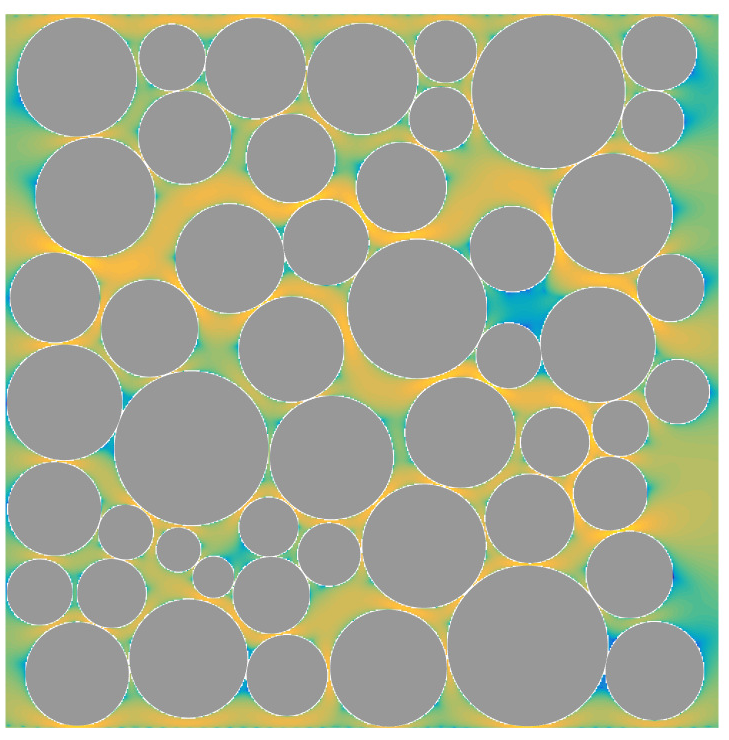
\includegraphics[height = 0.3 \textwidth]{./figs/vel_log_50b1}
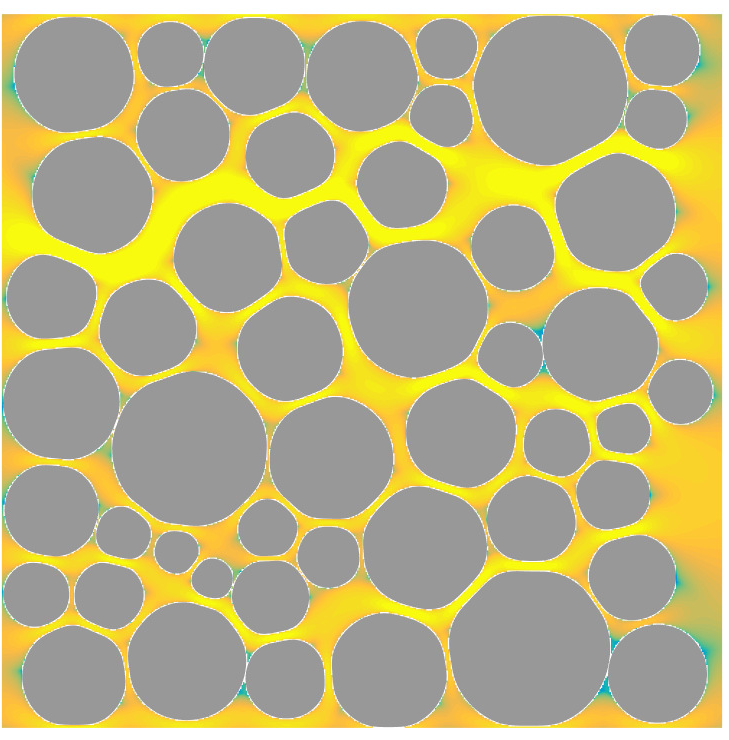
\includegraphics[height = 0.3 \textwidth]{./figs/vel_log_50b80}
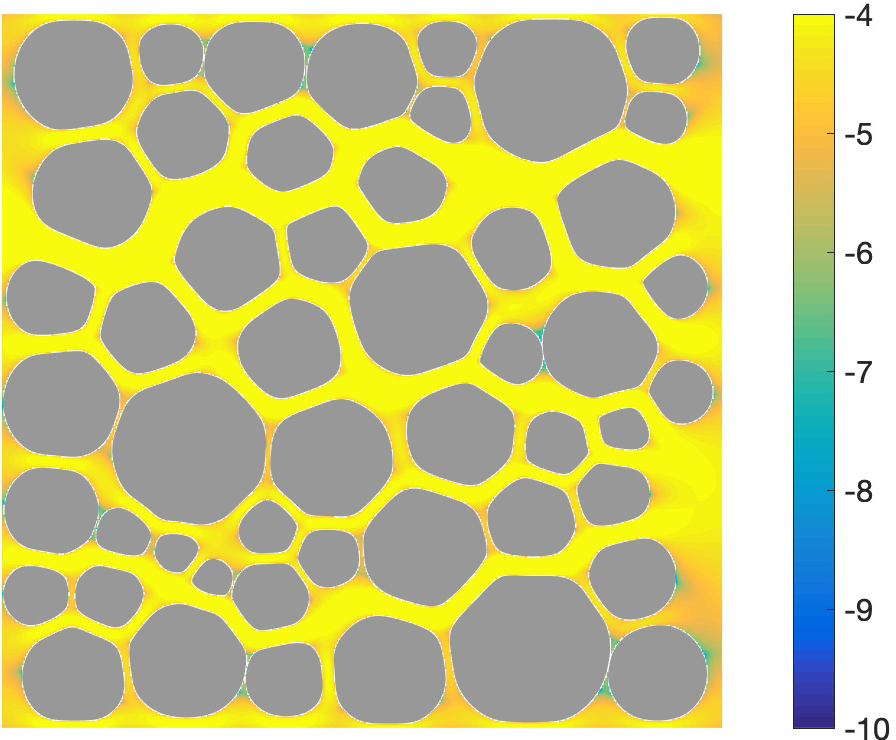
\includegraphics[height = 0.3 \textwidth]{./figs/vel_log_50b160}\\
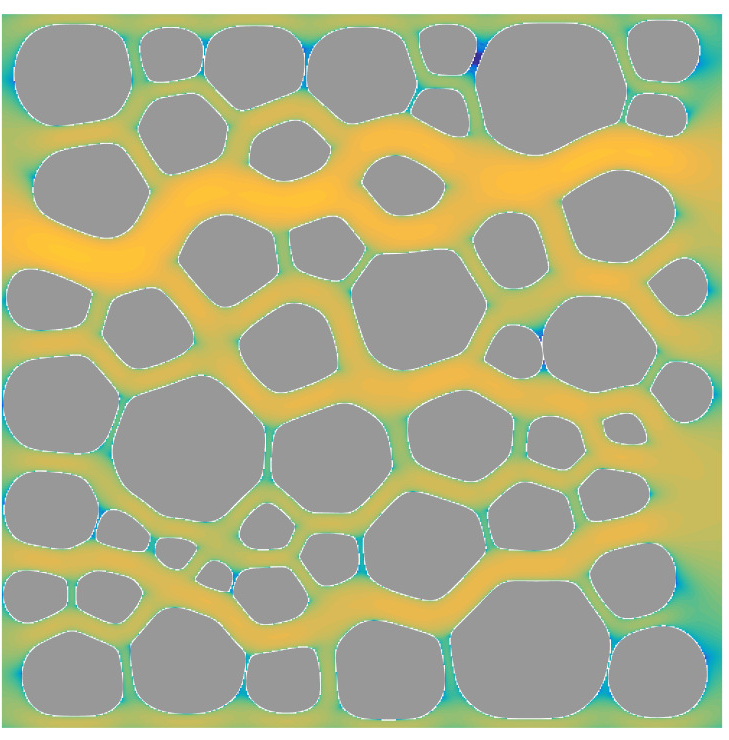
\includegraphics[height = 0.3 \textwidth]{./figs/vel_log_50b240}
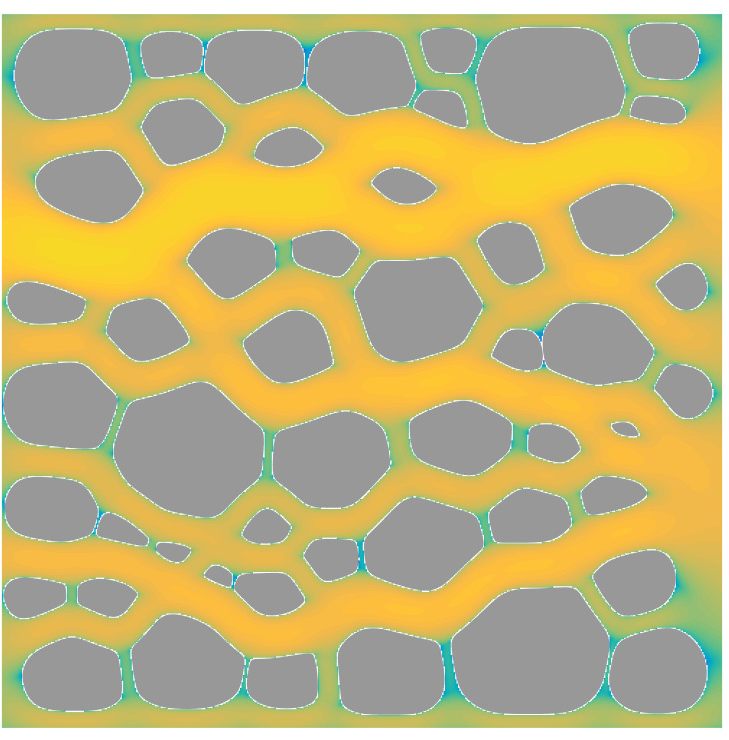
\includegraphics[height = 0.3 \textwidth]{./figs/vel_log_50b320}
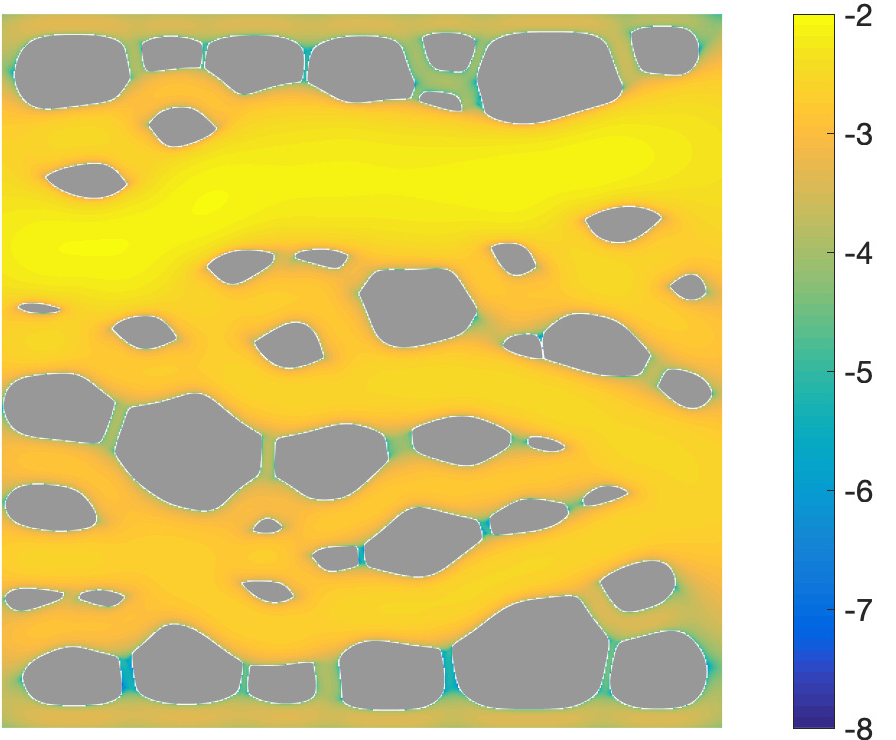
\includegraphics[height = 0.3 \textwidth]{./figs/vel_log_50b400}
\caption{\label{fig:Eroding50vel} Six evenly spaced snapshots of 50
eroding bodies.  The background velocity is a Hagen-Poiseuille flow with
a varying flow strength that corresponds to a constant pressure drop
across the channel. The color is the magnitude of the velocity in a
logarithmic scale. The flow velocity varies over several orders of
magnitude, the grains form irregular shapes with large aspect ratios,
and the geometry becomes channelized and anisotropic.}
\end{center}
\end{figure}

This study consists of two main undertakings: first, high-fidelity
simulations of eroding porous media, and, second, characterization of
tracer transport through the resulting eroded geometries. Our modeling
efforts build on previous work~\citep{ris-moo-chi-she-zha2012,
moore2013self, moo2017}, in particular recent numerical methods
developed to simulate erosion in the Stokes-flow
regime~\citep{qua-moo2018}. We, however, make key improvements to the
numerical methods to enable simulations of more realistic, dense
suspensions of eroding grains (figures~\ref{fig:Eroding50vel}
and~\ref{fig:Eroding50vort}).  Then, to characterize transport through
these configurations, we examine coarse-grained variables through
statistical analysis of tracer trajectories.

Owing to the scales present in groundwater flow~\citep{bea1972}, we
model the hydrodynamics with the two-dimensional incompressible Stokes
equations.  Meanwhile, individual grains erode at a rate proportional to
the hydrodynamic shear stress~\citep{wan-fel2004,
ris-moo-chi-she-zha2012, moore2013self, par-izu2000}.  We compute the
vorticity in the fluid bulk since, on solid boundaries, vorticity
reduces to shear and thus provides a convenient way to simultaneously
visualize local erosion rates and changes in the surrounding flow
(figure~\ref{fig:Eroding50vort}).  A variety of numerical methods for
the fluid solver are available including lattice-gas or lattice
Boltzmann~\citep{kop-kat-tim1996, dar-mcc1998}, finite
volumes~\citep{suo-liu-gan2019, den-ica-hid2018,
sie-ili-pri-riv-gua2019}, finite differences~\citep{leb-ded-dav-bou2007,
knu-car2005}, and cellular automata~\citep{rot1988}.  However,
simulating erosion requires a method that is high-order, can resolve
nearly-touching arbitrarily shaped grains, and can accurately compute
derivatives of the velocity field.  Since the governing equations are
linear and homogeneous, we address these challenges by converting the
fluid equations to a boundary integral equation (BIE).

\begin{figure}
\begin{center}
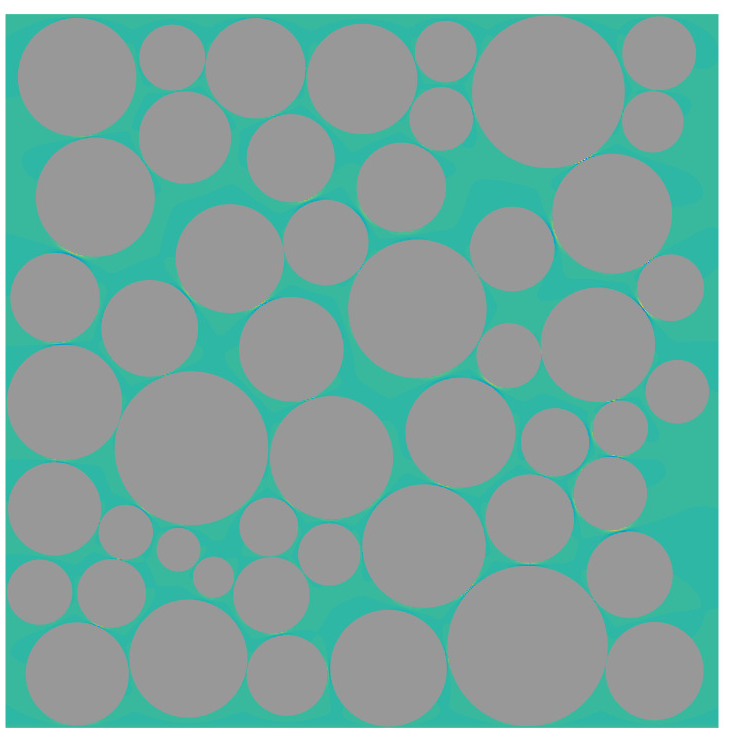
\includegraphics[height = 0.3 \textwidth]{./figs/vort_50b1}
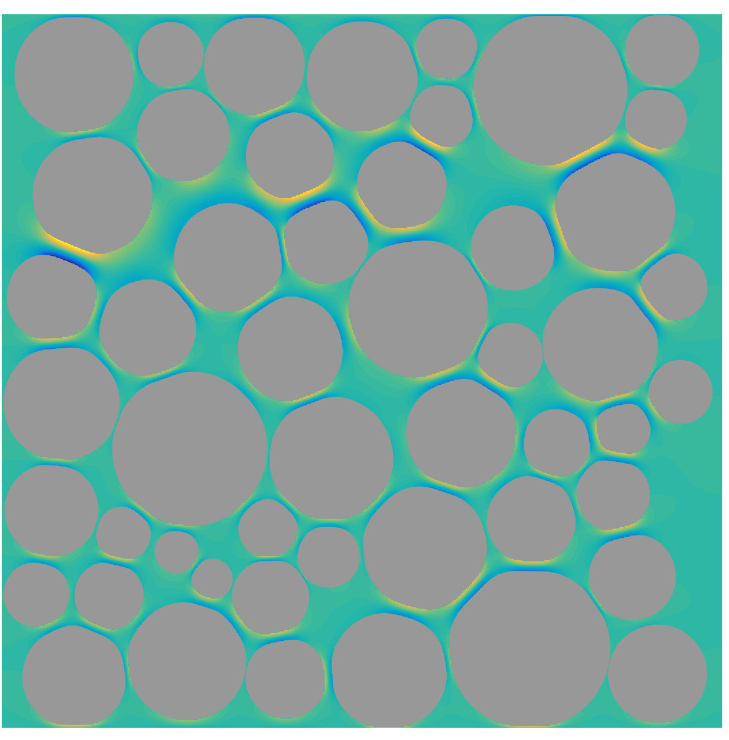
\includegraphics[height = 0.3 \textwidth]{./figs/vort_50b80}
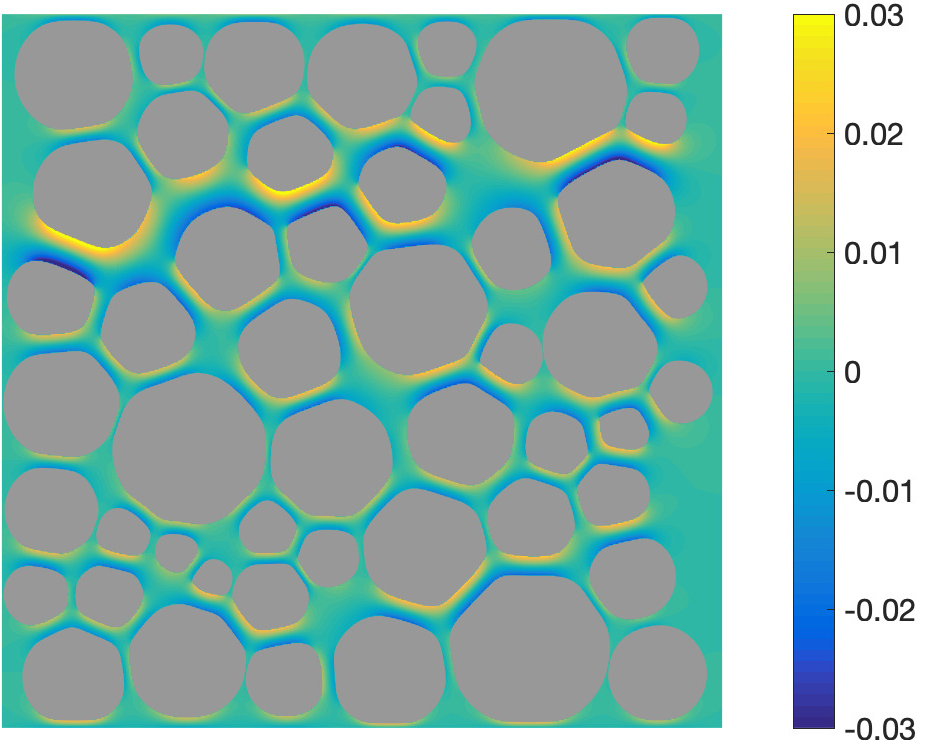
\includegraphics[height = 0.3 \textwidth]{./figs/vort_50b160}\\
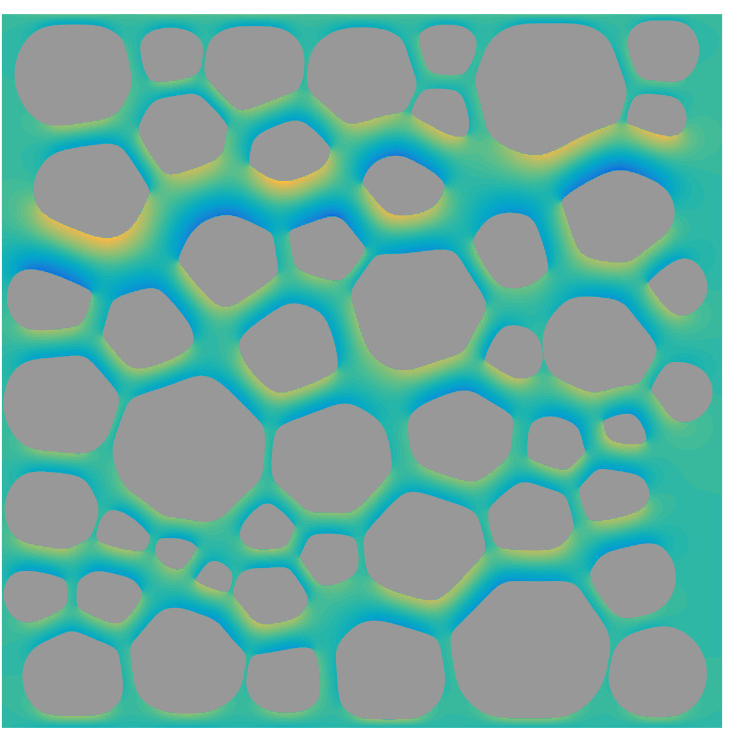
\includegraphics[height = 0.3 \textwidth]{./figs/vort_50b240}
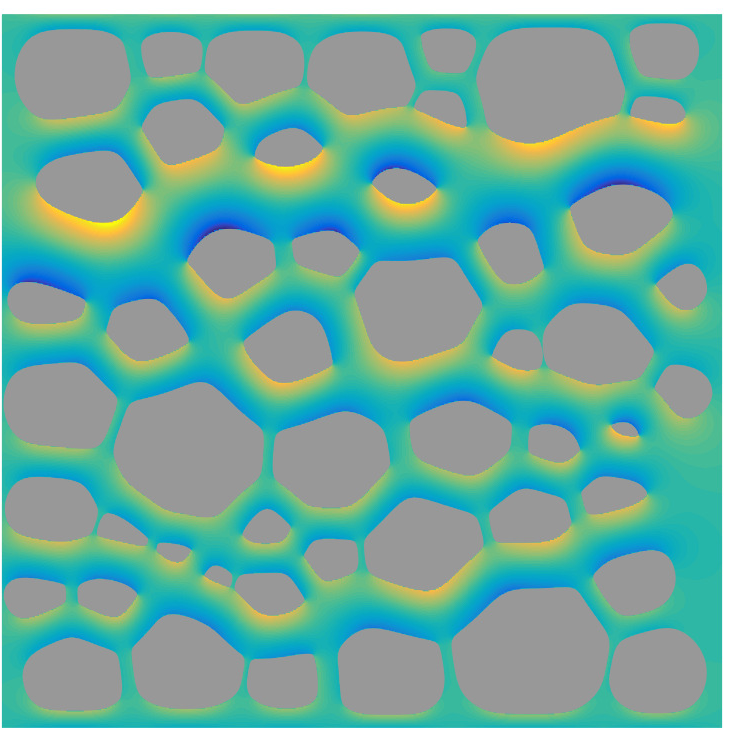
\includegraphics[height = 0.3 \textwidth]{./figs/vort_50b320}
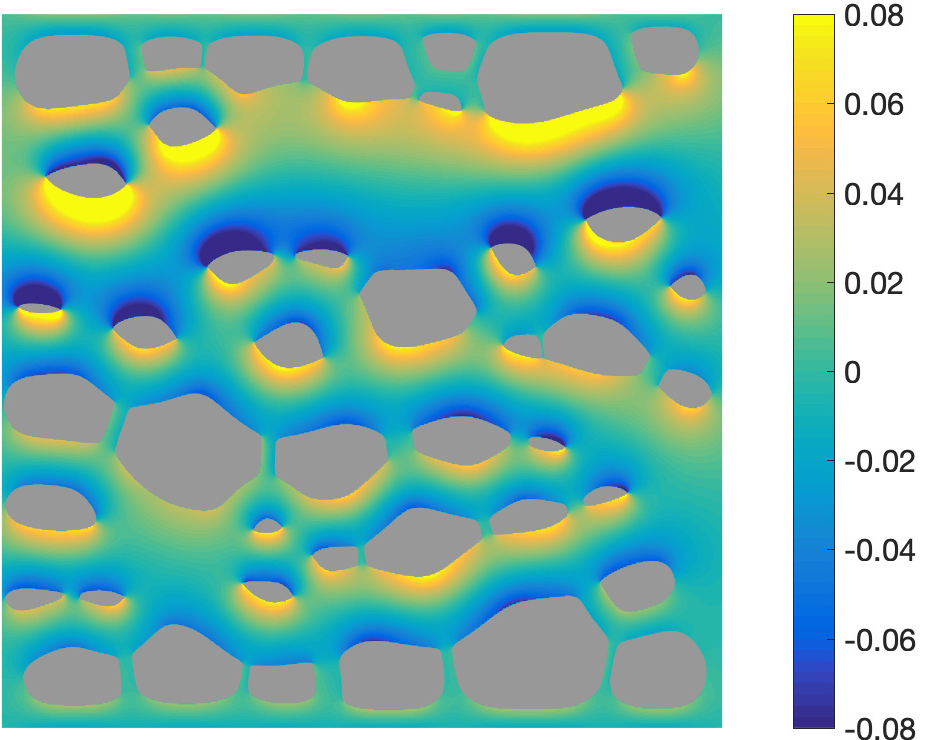
\includegraphics[height = 0.3 \textwidth]{./figs/vort_50b400}
\caption{\label{fig:Eroding50vort} The same six snapshots as
figure~\ref{fig:Eroding50vel}.  The color is the vorticity of the fluid.
Since the rate of erosion is equivalent to the magnitude of the
vorticity, erosion is fastest in the yellow and blue regions and slowest
in the green regions.}
\end{center}
\end{figure}

To compute stable simulations of erosion, we use high-order methods in
both space and time. The time integration method is unchanged from
previous work~\citep{qua-moo2018}.  We apply a mild regularization and a
smoothing term to eliminate numerical instabilities that can be
triggered by changes in sign of the shear stress, and we use a stable
second-order Runge-Kutta method applied to the {\thL}
coordinates~\citep{hou-low-she1994} of the eroding grains.  In this
work, we introduce a new quadrature method to resolve dense suspensions.
The accuracy of the trapezoid rule, which was used in previous work, is
adequate for bodies that are sufficiently separated~\citep{tre-wei2014}.
However, it loses accuracy whenever grains are in close contact.  One of
the earliest works to address quadrature methods for nearly-singular
integrands was developed by~\citet{bak-she1986}, and in recent years,
many other near-singular integration schemes have
followed~\citep{oja-tor2015, kli-tor2018, hel-oja2008a, bea-yin-wil2016,
bea-lai2001, klo-bar-gre-one2013}.  We use a Barycentric quadrature
method~\citep{bar2014, bar-wu-vee2015} since it is a non-intrusive
modification of the trapezoid rule, and the error is guaranteed to be
uniformly bounded.  We extend the original quadrature method to compute
the velocity gradient, which is needed to evaluate the shear stress and
the fluid vorticity.

To characterize transport through the resulting configurations, particle
trajectories must be computed. Depending on the application, microscale
transport can be modelled as pure advection~\citep{dea-qua-bir-jua2018,
leb-ded-dav-bou2007, cve-che-wen1996, puy-gou-den2019},
advection-diffusion~\citep{cus-hu-den1995, dag1987, den-ica-hid2018}, or
with a random walk~\citep{saf1959, bij-blu2006, ber-sch-sil2000}.  In
this work, we assume trajectories to be governed by pure advection
(ie.~no diffusion), so the particle trajectories are identical to the
streamlines. We compute trajectories $\ss(t)$ that are initialized at
$\ss_0$ by solving the advection equation
\begin{align}
  \frac{d\ss}{dt} = \uu(\ss,t), \quad \ss(0) = \ss_0,
  \label{eqn:tracers}
\end{align}
where $\uu$ is the fluid velocity.  Since there is no stiff diffusive
term, we solve~\eqref{eqn:tracers} with a fourth-order explicit
Runge-Kutta time stepping method.  In addition, the Barycentric
quadrature rule is used to accurately compute trajectories that are
close to an eroding grain. 
%We note that an alternative approach to
%compute trajectories is to form a distribution of velocities $\uu$ and
%use a continuous time random walk~\citep{mon-wei1965,
%den-cor-sch-ber2004, leb-den-car2008, ber-cor-den-sch2006}.

Once the streamlines are computed, we characterize transport by
analyzing three different metrics: the tortuosity, the anomalous
dispersion, and the pore size distribution.  The local tortuosity of a
streamline that connects the inlet to the outlet is defined as the
streamline's length normalized by the linear inlet-to-outlet distance.
In porous media, the local tortuosity can be greater than
1.5~\citep{kop-kat-tim1996, mat-kha-koz2008} or even
2~\citep{dud-koz-mat2011}, depending on several factors such as the
porosity. The tortuosity of a geometry is defined by averaging the local
tortuosity over all streamlines initialized at the inlet, and the
geometry's tortuosity characterizes average particle
motions~\citep{hak-com-den2019}.  To characterize spreading, the fluid
dispersion is computed by calculating the variance of the streamline
lengths. In porous media, this spreading is often
super-dispersive~\citep{kan-dea-nun-bij-blu-jua2014, cus-hu-den1995,
dea-leb-den-tar-bol-dav2013}. Since anomalous dispersion results from
streamlines spending time in both the high and low velocity
regimes~\citep{ber-sch2001}, it is crucial to accurately resolve
streamlines near grain boundaries, as achieved in this work.  Finally,
we construct the pore-size distribution throughout the erosion process.
These distributions are required to quantify velocity
distributions~\citep{ali-par-wei-bre2017, dea-qua-bir-jua2018},
channelization~\citep{sie-ili-pri-riv-gua2019},
connectivity~\citep{knu-car2005, wes-blo-gra2001}, and to develop
network models~\citep{bry-kin-mel1993, bry-mel-cad1993, bij-blu2006}. 

%%%%%%%%%%%%%%%%%%%%%%%%%%%%%%%%%%%%%%%%%%%%%%%%%%%%%%%%%%%%%%%%%%%%%%%
%\subsection{Contributions}
%Our first contribution is extending the Barycentric quadrature rule
%of~\citet{bar-wu-vee2015} to accurately compute velocity gradients
%associated with Stokes flow. This new quadrature rule permits accurate
%and stable simulations of erosion, and, moreover, enables visualization
%of the vorticity field throughout.
%
%Our second contribution is computing and analyzing trajectories in
%eroded geometries.  These trajectories are formed by combining the
%Barycentric quadrature rule and a fourth-order Runge-Kutta method. Then,
%they are used to compute tortuosities and dispersion rates of eroded
%geometries. Finally, we examine the effect of erosion on the pore size
%distribution.

%%%%%%%%%%%%%%%%%%%%%%%%%%%%%%%%%%%%%%%%%%%%%%%%%%%%%%%%%%%%%%%%%%%%%%%
%\subsection{Limitations}
%As in our previous work~\citep{qua-moo2018}, we consider two-dimensional
%immobile eroding grains. However, this work does not limit the proximity
%of  grains. Compared to our previous work, we are able to simulate much
%denser suspensions with a comparable number of discretization points and
%without upsampling.  While we do investigate transport in this work, we
%only consider passive particles that are advected by the flow.  To model
%other physical processes, such as contaminant transport, we plan to
%simulate a finite Peclet number advection-diffusion equation in eroded
%geometries.

%%%%%%%%%%%%%%%%%%%%%%%%%%%%%%%%%%%%%%%%%%%%%%%%%%%%%%%%%%%%%%%%%%%%%%%
%\subsection{Outline of the Paper}
This paper is organized as follows. In section~\ref{sec:formulation}, we
summarize the erosion model that is described in more detail in previous
work~\citep{qua-moo2018}.  In section~\ref{sec:DLP}, we recast all the
governing equations as layer potentials defined in both $\RR^2$ and in
$\CC$.  Section~\ref{sec:transport} describes measures for
characterizing the geometry and transport. Section~\ref{sec:method}
describes the numerical methods, with special attention paid to the new
quadrature method for computing the shear stress and the vorticity.
Section~\ref{sec:results} presents numerical examples for a variety of
dense packings of bodies.  Finally, concluding remarks are made in
section~\ref{sec:conclusions}.

%%%%%%%%%%%%%%%%%%%%%%%%%%%%%%%%%%%%%%%%%%%%%%%%%%%%%%%%%%%%%%%%%%%%%%%
\section{Governing Equations}
\label{sec:formulation}
%%%%%%%%%%%%%%%%%%%%%%%%%%%%%%%%%%%%%%%%%%%%%%%%%%%%%%%%%%%%%%%%%%%%%%%
We start by defining the main variables used to model erosion.  We only
briefly summarize the model, and a more detailed description can be
found in previous work~\citep{qua-moo2018}.  We consider flows inside a
confined geometry $\Omega$ that contains $M$ eroding bodies with
boundaries $\gamma_\ell$, $\ell = 1,\ldots,M$.  The boundary of the
fluid domain is $\bd \Omega = \Gamma \cup \gamma_1 \cup \cdots \cup
\gamma_M$, where $\Gamma$ is the outer boundary, taken to be a slightly
smoothed version of the boundary of $[-3,3] \times [-1,1]$.  We only
place eroding bodies in $[-1,1] \times [-1,1]$ to create a buffer region
for the flow profile imposed at the inlet to transition to the more
complex flow intervening between the bodies. On each eroding body, $\nn$
is the normal vector pointing into the body, and $\ss$ is the unit
tangent vector pointing in the counterclockwise direction.  The normal
vector on $\Gamma$ is the outward unit normal.  Neglecting inertial
forces, the governing equations are
\begin{equation}
\label{eqn:erosionModel}
  \begin{split}
    \mu \Delta \uu = \grad p, &\hspace{20pt} \xx \in \Omega, \gap 
      &&\mbox{\em conservation of momentum}, \\
    \grad \cdot \uu = 0, &\hspace{20pt} \xx \in \Omega, \gap 
      &&\mbox{\em conservation of mass}, \\
    \uu = \mathbf{0}, &\hspace{20pt} \xx \in \gamma, \gap 
      &&\mbox{\em no slip on the eroding bodies}, \\
    \uu = \UU, &\hspace{20pt} \xx \in \Gamma, \gap 
      &&\mbox{\em outer wall velocity}, \\
    \Vn = \CE \, \abs{\tau}, &\hspace{20pt} \xx \in \gamma,
      &&\mbox{\em erosion model}.
  \end{split}
\end{equation}
Here, $\uu$ is the fluid velocity, $p$ is the pressure, $\UU$ is a
prescribed Hagen-Poiseuille velocity field, $\Vn$ is the normal velocity
of $\gamma$, and
\begin{align}
  \tau = -(\nabla \uu + \nabla \uu^T) \nn \cdot \ss
  \label{eqn:shearStress}
\end{align}
is the shear stress on $\gamma$. We simulate erosion by alternating
between solving the fluid equations and advancing the eroding grains.
The strength of $\UU$ is adjusted at each time step to achieve a
constant pressure drop across the channel.

%%%%%%%%%%%%%%%%%%%%%%%%%%%%%%%%%%%%%%%%%%%%%%%%%%%%%%%%%%%%%%%%%%%%%%%
\section{Boundary Integral Equation Formulation}
\label{sec:DLP}
%%%%%%%%%%%%%%%%%%%%%%%%%%%%%%%%%%%%%%%%%%%%%%%%%%%%%%%%%%%%%%%%%%%%%%%
Since we require accurate solutions of the incompressible Stokes
equations in complex two-dimensional geometries, we reformulate the
equations as a BIE.  This has the advantage that only the
one-dimensional boundary of the domain must be discretized, and, with
appropriate quadrature formulas and fast summation methods, the result
is a high-fidelity numerical simulation with near-optimal computational
complexity.

%%%%%%%%%%%%%%%%%%%%%%%%%%%%%%%%%%%%%%%%%%%%%%%%%%%%%%%%%%%%%%%%%%%%%%%
\subsection{Double-Layer Potential Formulation in $\RR^2$}
%%%%%%%%%%%%%%%%%%%%%%%%%%%%%%%%%%%%%%%%%%%%%%%%%%%%%%%%%%%%%%%%%%%%%%%
Applying the same approach as our previous work~\citep{qua-moo2018}, we
start with the double-layer potential 
\begin{align}
  \DDD[\eeta](\xx) = \int_{\bd\Omega} D(\xx,\yy) \eeta(\yy)\, ds_\yy = 
  \frac{1}{\upi}\int_{\bd\Omega} 
    \frac{\rr \cdot \nn}{\rho^2} \frac{\rr \otimes \rr}{\rho^2}
    \eeta(\yy) \, ds_\yy, \quad \xx \in \Omega,
  \label{eqn:velocityDLP}
\end{align}
where $D$ is the kernel of the integral operator, $\rr = \xx - \yy$,
$\rho = \|\rr\|$, $\nn$ is the unit outward normal at $\yy$, and $\eeta$
is an unknown density function.  The double-layer potential is a
solution of the incompressible Stokes equations, but it cannot represent
all the solutions. Therefore, we complete the integral equation
formulation by adding the $M$ Stokeslets and rotlets~\citep{pow-mir1987}
\begin{align}
  S[\llambda_\ell,\cc_\ell](\xx) = \frac{1}{4\upi} \left( 
    -\log \rho \II + \frac{\rr \otimes \rr}{\rho^2}
    \right)\llambda_\ell, \quad
  R[\xi_\ell,\cc_\ell](\xx) = \frac{\rr^\perp}{\rho^2} \xi_\ell,
  \quad \ell=1,\ldots,M,
\end{align}
where $\rr = \xx - \cc_\ell$, $\cc_\ell$ is a point inside the
$\ell^{th}$ eroding body, $\rr^\perp = (r_2,-r_1)$, and $\rho =
\|\rr\|$. Here, $\llambda_\ell$ and $\xi_\ell$ are the Stokeslet and
rotlet strengths, respectively, corresponding to the $\ell^{th}$ body.
Then, for any sufficiently smooth geometry $\Omega$, the solution of the
incompressible Stokes equation with a Dirichlet boundary condition $\ff$
is
\begin{align}
  \uu(\xx) = \DDD[\eeta](\xx) + 
    \sum_{\ell=1}^M S[\llambda_\ell,\cc_\ell](\xx) + 
    \sum_{\ell=1}^M R[\xi_\ell,\cc_\ell](\xx), \quad \xx \in \Omega,
\end{align}
where the density function, Stokeslets, and rotlets satisfy
\begin{subequations}
\label{eqn:BIE}
\begin{alignat}{3}
  \ff(\xx) &= -\frac{1}{2}\eeta(\xx) + \DDD[\eeta](\xx) + 
    \NN_0[\eeta](\xx) \nonumber \\
    &\quad + \sum_{\ell=1}^M S[\llambda_\ell,\cc_\ell](\xx) + 
    \sum_{\ell=1}^M R[\xi_\ell,\cc_\ell](\xx), 
    \quad &&\qquad\xx \in \bd\Omega, \\
  \llambda_\ell &= \frac{1}{2\upi} \int_{\gamma_\ell} 
    \eeta(\yy)\, ds_\yy, &&\qquad \ell = 1,\ldots,M, \\
  \xi_\ell &= \frac{1}{2\upi} \int_{\gamma_\ell}
    (\yy - \cc_\ell)^\perp \cdot \eeta(\yy)\, ds_\yy, 
    &&\qquad \ell = 1,\ldots,M.
\end{alignat}
\end{subequations}
Here, the null space associated with the flux-free condition of $\ff$ is
addressed with  $\NN_0$ which is the integral operator with kernel
$N_0(\xx,\yy) = \nn(\xx) \otimes \nn(\yy)$, $\xx,\yy \in \Gamma$.  In
this work, $\ff$ is the prescribed velocity, which is equal to $\UU$ on
the outer wall, $\Gamma$, and equal to zero on the eroding bodies,
$\gamma_\ell$, $\ell=1,\ldots,M$.

Once~\eqref{eqn:BIE} is solved for the density function $\eeta$, the
Stokeslets $\llambda_\ell$, and the rotlets $\xi_\ell$, we are able to
compute, for $\xx \in \Omega$, the deformation tensor, pressure, and
vorticity, defined respectively as
\begin{align}
  \label{eqn:deformationDLP} 
  \ssigma(\xx) &= \int_{\bd\Omega} \mathbf{D}_{\ssigma}(\xx,\yy) 
      \eeta(\yy) ds_{\yy} 
  = \frac{1}{2\upi}\int_{\bd\Omega} \left(
    2\frac{\rr \cdot \nn}{\rho^2} \frac{\rr \cdot \eeta}{\rho^2} \II + 
    \frac{\rr \cdot \eeta}{\rho^4} (\nn \otimes \rr + \rr \otimes \nn) 
    \right. \nonumber \\
    & \qquad\qquad\qquad\qquad \left.
    +\frac{\rr \cdot \nn}{\rho^4} (\eeta \otimes \rr + \rr \otimes \eeta) - 
    8\frac{(\rr \cdot \nn)(\rr \cdot \eeta)}{\rho^6}(\rr \otimes \rr)
    \right) \, ds_\yy, \\
%
  \label{eqn:pressureDLP}
  p(\xx) &= \int_{\bd\Omega} D_{p}(\xx,\yy) 
      \eeta(\yy) ds_{\yy} 
  = -\frac{1}{\upi}\int_{\bd\Omega} \frac{1}{\rho^2}
    \left(I - 2 \frac{\rr \otimes \rr}{\rho^2}\right) \nn \cdot
      \eeta(\yy)\,ds_\yy, \\
%
  \label{eqn:vorticityDLP} 
  \omega(\xx) &= \int_{\bd\Omega} D_{\omega}(\xx,\yy) 
      \eeta(\yy) ds_{\yy} 
  = -\frac{1}{\upi} \int_{\bd\Omega}
    \frac{(\rr \cdot \nn^\perp) + (\rr \cdot \nn)}{\rho^4} 
      (\rr \cdot \eeta) \, ds_\yy.
\end{align}
Since the deformation tensor of the double-layer potential is
discontinuous across $\bd\Omega$, the jump term 
\begin{align}
  \frac{1}{2} \left(\pderiv{\eeta}{\ss} \cdot \ss \right) \left[
    \begin{array}{cc}
      s_x^2 - s_y^2 & 2s_x s_y \\ 2s_x s_y & s_y^2 - s_x^2
    \end{array}
  \right],
  \label{eqn:deformationJump}
\end{align}
must be added to $\ssigma(\xx)$ for $\xx \in \bd\Omega$.  Finally, the
Stokeslets and rotlets do not exhibit any jumps across $\gamma$, so the
associated components of the deformation tensor, pressure, and vorticity
are straightforward to compute~\citep{poz1992}.  Having computed the
deformation tensor on $\gamma$, the shear stress is computed using
equation~\eqref{eqn:shearStress}.  

%%%%%%%%%%%%%%%%%%%%%%%%%%%%%%%%%%%%%%%%%%%%%%%%%%%%%%%%%%%%%%%%%%%%%%%
\subsection{Cauchy Integral Representation of the Double-Layer
Potential}
\label{sec:DLPcomplex}
%%%%%%%%%%%%%%%%%%%%%%%%%%%%%%%%%%%%%%%%%%%%%%%%%%%%%%%%%%%%%%%%%%%%%%%
In
equations~\eqref{eqn:velocityDLP},~\eqref{eqn:deformationDLP},~\eqref{eqn:pressureDLP},
and~\eqref{eqn:vorticityDLP}, the fluid velocity, deformation tensor,
pressure, and vorticity are all written as layer potentials in $\RR^2$.
However, the quadrature method we introduce in section~\ref{sec:method}
requires a complex-valued representation of the layer potentials for the
velocity, deformation tensor, and vorticity. The first step to form a
complex representation is to write the Laplace double-layer potential as
the complex integral
\begin{align}
  \DD[\eeta](\xx) = \frac{1}{2\upi} \int_{\bd\Omega} 
    \frac{\rr \cdot \nn}{\rho^2}\eeta(\yy)\, ds_\yy = \Real (v(x)),
\end{align}
where
\begin{align}
  v(x) = \frac{1}{2\upi i} \int_{\bd\Omega}
    \frac{\eta(y)}{x - y} \, dy, \quad x \in \Omega.
  \label{eqn:laplaceComplex}
\end{align}
Here $x = x_1 + i x_2,y = y_1 + i y_2 \in \CC$ are the complex
counterparts of $\xx = (x_1,x_2),\yy = (y_1,y_2) \in \RR^2$, and $\eta =
\eta_1 + i \eta_2$ is the complex counterpart of $\eeta =
(\eta_1,\eta_2)$. Therefore, depending on the formulation of the layer
potential, $\Omega$ is being interpreted as a subset of $\RR^2$ or
$\CC$. Equation~\eqref{eqn:laplaceComplex} is converted to a Cauchy
integral by first finding the boundary data of $v$.  Assuming that
$\Omega$ is a simply-connected interior domain, the boundary data of $v$
satisfies the Sokhotski-Plemelj jump relation
\begin{align}
  \label{eqn:SPrelation}
  v(x) = - \frac{1}{2} \eta(x) + \frac{1}{2\upi i} \int_{\bd\Omega}
    \frac{\eta(y)}{x-y}\, dy, \quad x \in \Omega.
\end{align}
For exterior domains, the jump term changes from $-1/2$ to $1/2$, and
for multiply-connected domains, such as a porous media, $\bd\Omega$ is
decomposed into its different connected components and the appropriate
jump relation is applied.  Having computed the boundary data of the
holomorphic function $v$, by the Cauchy integral theorem we have
\begin{subequations}
  \label{eqn:cauchy}
  \begin{alignat}{3}
  v(x) &= \frac{1}{2\upi i}\int_{\bd\Omega} 
    \frac{v(y)}{y-x} \,dy, \\
  v'(x) &= \frac{1}{2\upi i} \int_{\bd\Omega}
    \frac{v(y)}{(y-x)^2} \, dy, \\
  v''(x) &= \frac{1}{\upi i} \int_{\bd\Omega}
    \frac{v(y)}{(y-x)^3} \, dy,
  \end{alignat}
\end{subequations}
for $x \in \Omega$.  Since $v(x)$ depends on the complex-valued density
function $\eta$, we use the notation $v[\eta](x)$ for the holomorphic
function defined in equation~\eqref{eqn:laplaceComplex}, and its first
two derivatives are written as $v'[\eta](x)$ and $v''[\eta](x)$.  
  
Finally, the Stokes double-layer potential~\eqref{eqn:velocityDLP} can
be written using a Laplace double-layer
potential~\eqref{eqn:laplaceComplex} and its gradients 
\begin{equation}
  \label{eqn:Stokes2Laplace}
  \begin{aligned}
    \DDD[\eeta](\xx) &= 
      \frac{1}{2\upi} \int_{\bd\Omega} 
        \frac{\nn}{\rho^2} (\rr \cdot \eeta) \, ds_\yy + 
      \frac{1}{2\upi} \nabla \int_{\bd\Omega}
        \frac{\rr \cdot \nn}{\rho^2} (\yy \cdot \eeta) \, ds_\yy \\
      &- \frac{1}{2\upi} x_1 \nabla \int_{\bd\Omega}
        \frac{\rr \cdot \nn}{\rho^2}\eta_1(\yy) \, ds_\yy -
      \frac{1}{2\upi} x_2 \nabla \int_{\bd\Omega}
        \frac{\rr \cdot \nn}{\rho^2}\eta_2(\yy) \, ds_\yy.
  \end{aligned}
\end{equation}
Therefore, the Stokes double-layer potential can be written as a sum of
Cauchy integrals and its first derivative~\citep{bar-wu-vee2015}
\begin{equation}
  \begin{aligned}
    u_1(x) &= \Real (v[\psi_1](x)) + \Real (v'[y\cdot\eta](x)) 
             -x_1\Real (v'[\eta_1](x)) - x_2\Real (v'[\eta_2](x)), \\
    u_2(x) &= \Real (v[\psi_2](x)) - \Imag (v'[y\cdot\eta](x)) 
         +x_1\Imag (v'[\eta_1](x)) + x_2\Imag (v'[\eta_2](x)),
  \end{aligned}
  \label{eqn:cauchyVelocity}
\end{equation}
where $y \cdot \eta = y_1 \eta_1 + i y_2 \eta_2 \in \CC$, 
\begin{align} 
  \psi_1=(\eta_1+i\eta_2)\frac{\Real(n)}{n}, \quad
  \psi_2=(\eta_1+i\eta_2)\frac{\Imag(n)}{n},
\end{align}
and $n \in \CC$ is the complex counterpart of the outward unit normal
$\nn \in \RR^2$.

%%%%%%%%%%%%%%%%%%%%%%%%%%%%%%%%%%%%%%%%%%%%%%%%%%%%%%%%%%%%%%%%%%%%%%%
\subsection{Cauchy Integral Representation for the Gradient of the
Double-Layer Potential}
\label{sec:gradDLPcomplex}
%%%%%%%%%%%%%%%%%%%%%%%%%%%%%%%%%%%%%%%%%%%%%%%%%%%%%%%%%%%%%%%%%%%%%%%
Computing the shear stress and vorticity requires a complex-valued layer
potential representation of the velocity gradient.  The deformation
tensor at $x \in \Omega$ is found by computing the derivatives of the
expressions for $u_1$ and $u_2$ in equation~\eqref{eqn:cauchyVelocity}  
\begin{equation}
\label{eqn:cauchyGradient}
  \begin{aligned}
    \pderiv{u_1}{x_1} &= +\Real (v'[\psi_1](x)) + 
    \Real (v''[y\cdot\eta](x)) - \Real (v'[\eta_1](x)) \\
    &- x_1\Real (v''[\eta_1](x)) - x_2\Real (v''[\eta_2](x)), \\
    \pderiv{u_1}{x_2} &= - \Imag (v'[\psi_1](x)) - 
    \Imag (v''[y\cdot\eta](x)) + x_1\Imag (v''[\eta_1](x)) \\
    &- \Real (v'[\eta_2](x)) + x_2\Imag (v''[\eta_2](x)), \\
    \pderiv{u_2}{x_1} &= +\Real (v'[\psi_2](x)) - 
    \Imag (v''[y\cdot\eta](x)) + \Imag (v'[\eta_1](x))  \\
    &+ x_1\Imag (v''[\eta_1](x)) + x_2\Imag (v''[\eta_2](x)), \\
    \pderiv{u_2}{x_2} &= -\Imag (v'[\psi_2](x)) - 
    \Real (v''[y\cdot\eta](x)) + x_1\Real (v''[\eta_1](x)) \\
    &+ \Imag (v'[\eta_2](x)) + x_2\Real (v''[\eta_2](x)).
  \end{aligned}
\end{equation}
The same expressions are used to compute the deformation tensor for $x
\in \bd\Omega$, except that the jump
condition~\eqref{eqn:deformationJump} is included.  Finally, to compute
the shear stress, the deformation tensor on $\bd\Omega$ is applied to
the normal and tangent vectors as in equation~\eqref{eqn:shearStress}.
The velocity gradient is also used to compute the vorticity in the fluid
bulk.  For $x \in \Omega$, the Cauchy integral representation of the
vorticity at $x \in \Omega$ is
\begin{align}
  \omega(x) = 
    \Real (v'[\psi_2](x)) + \Imag (v'[\psi_1](x))+ 
    \Real (v'[\eta_2](x))+ \Imag (v'[\eta_1](x)).
\end{align}

%%%%%%%%%%%%%%%%%%%%%%%%%%%%%%%%%%%%%%%%%%%%%%%%%%%%%%%%%%%%%%%%%%%%%%%
\section{Transport, Tracers, and Tortuosity}
\label{sec:transport}
%%%%%%%%%%%%%%%%%%%%%%%%%%%%%%%%%%%%%%%%%%%%%%%%%%%%%%%%%%%%%%%%%%%%%%%
Erosion in porous media leads to particular phenomena such as
channelization~\citep{berhanu2012shape}, and we are interested in
characterizing transport in such geometries.  In our previous
work~\citep{qua-moo2018}, we examined the effect of erosion on the area
fraction, flow rate, and the total drag.  However, to characterize
macroscopic signatures of the transport, other quantities must be
examined.  Here, we compute the anomalous dispersion rate, the
tortuosity, and the distribution of the pore sizes.  The first two
metrics can be defined in terms of streamlines governed by the
autonomous advection equation~\eqref{eqn:tracers}.

%%%%%%%%%%%%%%%%%%%%%%%%%%%%%%%%%%%%%%%%%%%%%%%%%%%%%%%%%%%%%%%%%%%%%%%
\subsection{Anomalous Dispersion}
\label{sec:dispersion}
%%%%%%%%%%%%%%%%%%%%%%%%%%%%%%%%%%%%%%%%%%%%%%%%%%%%%%%%%%%%%%%%%%%%%%%
The spreading of fluid in a porous media is often characterized in terms
of anomalous dispersion~\citep{kla-rad-sok2008, den-cor-sch-ber2004}.
The anomalous dispersion rate depends on the porosity and
permeability~\citep{koc-bra1988}, but is also affected by the
distribution and shape of the grains. We calculate the anomalous
dispersion rates by analyzing the streamlines governed by
equation~\eqref{eqn:tracers} in eroded geometries. Given a set of $N_p$
trajectories, we define $\lambda_j(t)$ to be the arclength of the
trajectory
\begin{align}
  \lambda_j(t) = \int_{0}^t \|\ss'_j(\tilde{t})\|\, d\tilde{t}, 
    \quad j=1,\ldots,N_p.
\end{align}
Then, the first and second ensemble moments are
\begin{align}
  \label{eqn:moments}
  \langle \lambda \rangle (t) = 
    \frac{1}{N_p} \sum_{j=1}^{N_p} \lambda_j(t), \quad 
    \sigma_\lambda^2(t) = \frac{1}{N_p} \sum_{j=1}^{N_p}
    \left[\lambda_j(t) - \langle \lambda \rangle(t) \right]^2,
\end{align}
and $\sigma_\lambda$ characterizes particle dispersion.  At early times,
the particles have not explored much of the geometry, and we expect a
ballistic motion $\sigma_\lambda \sim t$.  However, as the particles
pass the grains, their trajectories are altered, and we expect that
$\sigma_\lambda \sim t^\alpha$, with $\alpha \in (0.5,1)$, indicating
that the flow is super-dispersive.

To establish an anomalous dispersion rate, the trajectories must pass
several grains so that an asymptotic regime is reached. The geometries
that we consider are too short to observe asymptotic dispersion, so we
use a reinsertion method to form longer trajectories. Similar to the
work of others~\citep{dea-qua-bir-jua2018, puy-gou-den2019}, once a
particle reaches the outlet of the porous region, it is reinserted at
the inlet.  To minimize errors caused by reinsertion, the particle is
initialized at the discretization point that has the closest velocity to
the particle's velocity at the outlet.  After a single trajectory is
formed, it has undergone a collection of reinsertions.  Then, as a
post-processing step, the trajectory is made continuous by attaching the
tail of each segment to the origin of the next segment.

We consider trajectories in an open channel so that they can be compared
to trajectories in eroded geometries with large permeability.  The
trajectory originating at $(s_1(0),s_2(0))$ is
\begin{align}
  s_1(t) = (1-s_2(0)^2)t + s_1(0), \quad
  s_2(t) = s_2(0).
\end{align}
Averaging over $s_2(0) \in [-1,1]$, the first and second ensemble
moments are
\begin{align}
  \langle \lambda \rangle (t) = \frac{2}{3}t, \quad 
    \sigma_\lambda^2(t) = \frac{4}{45}t^2.
\end{align}
In section~\ref{sec:results}, we compare the second moment in an open
channel with the trajectories in an eroded geometry.

%%%%%%%%%%%%%%%%%%%%%%%%%%%%%%%%%%%%%%%%%%%%%%%%%%%%%%%%%%%%%%%%%%%%%%%
\subsection{Tortuosity}
%%%%%%%%%%%%%%%%%%%%%%%%%%%%%%%%%%%%%%%%%%%%%%%%%%%%%%%%%%%%%%%%%%%%%%%
The tortuosity is a dimensionless number that quantifies the amount of
twisting of streamlines. Unlike the dispersion calculations, we do not
use reinsertion to form long trajectories.  The local tortuosity is
\begin{align}
  \tau(y_0) = \frac{\lambda(y_0)}{d}.
  \label{eqn:localTort}
\end{align}
Here the streamline originates on the inlet cross-section $x=x_0$ at
$(x_0,y_0)$, and its arclength, $\lambda(y_0)$, is calculated until the
streamline passes the parallel outlet cross-section $x = x_0 + d$.  In
this work, we consider streamlines originating at $x=-1$ and terminating
at $x=1$, so $d=2$.  However, other choices for the terminal point when
computing the tortuosity are sometime used~\citep{dud-koz-mat2011}.  The
hydraulic tortuosity is defined by taking the average over all points on
the inlet cross-section
\begin{align}
  T = \frac{1}{d}\frac{\displaystyle\int_{S}u_1(x_0,y_0)\lambda(y_0)\,dy_0}
  {\displaystyle\int_{S}u_1(x_0,y_0)\,dy_0},
  \label{eqn:tortuosity1}
\end{align} 
where $S$ is the inlet cross-section $x = -1$, $u_1(y_0)$ is the
$x$-component of the velocity at the initial point of the streamline,
and $d=2$ is the distance between the inlet and outlet.  Note that $T
\geq 1$, and $T=1$ only if no grains are present.

The tortuosity can also be computed with an area integral. Assuming that
the flow is incompressible and not re-entrant, meaning that all
streamlines connect the two cross-sections, the tortuosity in
equation~\eqref{eqn:tortuosity1} is equivalent
to~\citep{dud-koz-mat2011}
\begin{align}
  T = \frac{\displaystyle\int_\Omega \|\uu(\yy)\|\, d\yy}
           {\displaystyle\int_\Omega u_1(\yy)\, d\yy},
  \label{eqn:tortuosity2}
\end{align}
where $\Omega$ is the fluid region between the inlet and outlet
cross-sections.  Recirculation zones are possible in viscous
fluids~\citep{hig1985}, but they are very small in the examples we
consider and have a negligible effect on the tortuosity.  Since
equation~\eqref{eqn:tortuosity2} does not require the additional work of
computing particle trajectories at every time step, we use this
definition for the majority of the tortuosity calculations.  However, we
do compare the two definitions for the tortuosity at several porosities
in section~\ref{sec:results}.

There have been efforts to relate the tortuosity, $T$, to the porosity,
$\phi$.  For example,~\citet{mat-kha-koz2008} propose the
models
\begin{subequations}
  \label{eqn:tortuosityModels}
  \begin{align}
    \widehat{T}(\phi) &= \phi^{-p}, \\
    \widehat{T}(\phi) &= 1-p \log \phi, \\
    \widehat{T}(\phi) &= 1+p (1-\phi), \\
    \widehat{T}(\phi) &= (1+p (1-\phi))^2, 
  \end{align}
\end{subequations}
where $p>0$ is a fitting parameter.  In section~\ref{sec:results}, we
compare these four models with the tortuosity of eroding porous
geometries.

%%%%%%%%%%%%%%%%%%%%%%%%%%%%%%%%%%%%%%%%%%%%%%%%%%%%%%%%%%%%%%%%%%%%%%%
\subsection{Pore Throat Size}
\label{sec:throats}
%%%%%%%%%%%%%%%%%%%%%%%%%%%%%%%%%%%%%%%%%%%%%%%%%%%%%%%%%%%%%%%%%%%%%%%
While transport in porous media depends on the porosity, it also depends
on the placement of the grains.  In particular, grain placement affects
velocity scales~\citep{ali-par-wei-bre2017}, correlation
structures~\citep{leb-ded-dav-bou2007}, contaminant
transport~\citep{knu-car2005},
channelization~\citep{sie-ili-pri-riv-gua2019,berhanu2012shape}, and
pore network models~\citep{bry-kin-mel1993, bry-mel-cad1993,
bij-blu2006}. To characterize the grain placement, we compute
distributions of pore sizes between neighboring grains.  To define
neighboring grains, we form a Delaunay triangulation using nodes placed
at the center of each eroding grain and at a collection of points around
the boundary of the porous media.  Then, we say that two grains are
neighbors if their centers share an edge of the
triangulation~\citep{dea-qua-bir-jua2018}. The pores of an eroded
geometry are illustrated in figure~\ref{fig:Eroding100gap}(a). We do not
consider pores between eroding bodies and the solid wall $\Gamma$, so
some of the grains near the porous region boundary only have two
neighbors. Having defined the pore sizes, we plot its distribution in
figure~\ref{fig:Eroding100gap}(b) and compare it with the Weibull
distribution, a distribution used by others to characterize pore
sizes~\citep{ioa-cha1993}.  In section~\ref{sec:Eroding100}, we
investigate the effect of erosion on the pore size distribution.
\begin{figure}
\begin{subfigure}[b]{0.5\textwidth}
\includegraphics*[height =0.8\linewidth]{./figs/triangulation_100b100}
\caption{}
\end{subfigure}
\begin{subfigure}[b]{0.5\textwidth}
\includegraphics*[height = 0.8\linewidth]{./figs/gap_hist100b100}
\caption{}
\end{subfigure}
\caption{\label{fig:Eroding100gap} (a) The pore sizes between
neighboring grains. Two grains are said to be neighbors if they share an
edge of a Delanuay triangulation with nodes at the center of each
eroding grain. (b) The distribution of the pore sizes of an eroded
geometry. The black curve is the Weibull distribution with the same
first two moments as the data.}
\end{figure}


%%%%%%%%%%%%%%%%%%%%%%%%%%%%%%%%%%%%%%%%%%%%%%%%%%%%%%%%%%%%%%%%%%%%%%%
\section{Numerical Methods}
\label{sec:method}
%%%%%%%%%%%%%%%%%%%%%%%%%%%%%%%%%%%%%%%%%%%%%%%%%%%%%%%%%%%%%%%%%%%%%%%
In line with our previous work~\citep{qua-moo2018}, we use two meshes to
simulate erosion. The integral equation is solved by discretizing the
boundary of the geometry at a set of collocation points distributed
equally in arclength (section~\ref{sec:spatialDiscretization}).
Depending on the proximity of the target point to the source points, the
quadrature rule is either the trapezoid rule or the Barycentric
quadrature rule (section~\ref{sec:bary}).  The criteria that determines
which quadrature method is applied is described in
section~\ref{sec:fmm}.  Once the shear stress is computed, the bodies
are eroded a single time step by using a {\thL}
discretization~\citep{hou-low-she1994, moore2013self}.  The time
stepping methods for erosion and passive particles are described in
section~\ref{sec:time}.

%%%%%%%%%%%%%%%%%%%%%%%%%%%%%%%%%%%%%%%%%%%%%%%%%%%%%%%%%%%%%%%%%%%%%%%
\subsection{Spatial Discretization}
\label{sec:spatialDiscretization}
%%%%%%%%%%%%%%%%%%%%%%%%%%%%%%%%%%%%%%%%%%%%%%%%%%%%%%%%%%%%%%%%%%%%%%%
Since we use a BIE formulation, we only need to discretize the
one-dimensional boundary of the domain.  Therefore, we easily resolve
complex geometries, and differentiation is performed with spectral
accuracy in Fourier space.  We discretize each eroding grain $\gamma_k$
with $N_\iin$ points and discretize the outer wall $\Gamma$ with
$N_\out$ points.  The $j^{th}$ discretization point on $\Gamma$ and
$\gamma_k$ are denoted by $\yy_j^0$ and $\yy^k_j$, respectively.  The
discretization points are initially distributed evenly in arclength, and
this equispacing is maintained throughout the entire simulation by using
the {\thL} formulation.  In addition, we apply
regularization~\citep{qua-moo2018} to slightly smooth the corners that
inevitably develop during erosion.

Given the discretization points of $\bd\Omega$, the trapezoid rule
results in the collocation method for~\eqref{eqn:BIE}
\begin{subequations}
\label{eqn:trapLinearSystem}
  \begin{alignat}{3}
  \UU_\ell &= \sum_{j=1}^{N_\out} 
    w^0_j D(\yy^0_\ell,\yy^0_j) \eeta_j^0 +
  \sum_{k=1}^M \sum_{j=1}^{N_\iin}
    w^k_j D(\yy^0_\ell,\yy^k_j) \eeta^k_j +
  \sum_{j=1}^{N_\out} w^0_j N_0(\yy^0_\ell,\yy^0_j)\eeta_j^0 
    \nonumber \\
  &+\sum_{k=1}^M S[\llambda_k,\cc_k](\yy^0_\ell) + 
  \sum_{k=1}^M R[\xi_k,\cc_k](\yy^0_\ell), 
  &&\hspace{-120pt}\ell = 1,\ldots,N_\out, \\
%
  \mathbf{0} &= \sum_{j=1}^{N_\out} 
    w^0_j D(\yy^m_\ell,\yy^0_j) \eeta_j^0 +
  \sum_{k=1}^M \sum_{j=1}^{N_\iin}
    w^k_j D(\yy^m_\ell,\yy^k_j) \eeta^k_j \nonumber \\
  &+\sum_{k=1}^M S[\llambda_k,\cc_k](\yy^m_\ell) + 
  \sum_{k=1}^M R[\xi_k,\cc_k](\yy^m_\ell),
    &&\hspace{-120pt}m=1,\ldots,M, \: \ell = 1,\ldots,N_\iin,  \\
%
  \llambda_m &= \frac{1}{2\upi} \sum_{j=1}^{N_\iin} 
    w_j^m \eeta^m_j, 
  &&\hspace{-120pt}m = 1,\ldots,M \\ 
  \xi_m &= \frac{1}{2\upi} \sum_{j=1}^{N_\iin} 
    w_j^m (\yy^m_j - \cc_m)^\perp \cdot \eeta^m_j,
  &&\hspace{-120pt}m=1,\ldots,M,
\end{alignat}
\end{subequations}
where $w^k_j$ are quadrature weights that depend on $N_\iin$, $N_\out$,
and the lengths of $\gamma^k$ and $\Gamma$, and $D$ is the kernel of the
Stokes double-layer potential defined in
equation~\eqref{eqn:velocityDLP}.  Since the kernel is smooth, the
diagonal terms $D(\yy_j^m,\yy_j^m)$ are replaced with the appropriate
curvature-dependent limiting term.  The linear
system~\eqref{eqn:trapLinearSystem} is a well-conditioned second-kind
integral equation and is solved iteratively with GMRES.  If the number
of discretization points is sufficiently large, then the solution
of~\eqref{eqn:trapLinearSystem} is an accurate approximation of the
density function, Stokeslets, and rotlets.   Then, if $\xx \in \Omega$
is sufficiently far from $\bd\Omega$, an approximation of the velocity,
deformation tensor, and vorticity due to the double-layer potential is
found by applying the trapezoid rule to \eqref{eqn:velocityDLP},
\eqref{eqn:deformationDLP}, and~\eqref{eqn:vorticityDLP}, respectively.
In particular,
\begin{align}
  \label{eqn:trap}
  \uu(\xx) &= \sum_{j=1}^{N_\out} w^0_j D(\xx,\yy^0_j) \eeta_j +
  \sum_{k=1}^M \sum_{j=1}^{N_\iin} w^k_j D(\xx,\yy^k_j) \eeta^k_j, \\
%
  \ssigma(\xx) &= \sum_{j=1}^{N_\out} w^0_j \mathbf{D}_\ssigma(\xx,\yy^0_j) \eeta_j +
  \sum_{k=1}^M \sum_{j=1}^{N_\iin} w^k_j \mathbf{D}_\ssigma(\xx,\yy^k_j)
  \eeta^k_j, \\
%
  w(\xx) &= \sum_{j=1}^{N_\out} w^0_j D_\omega(\xx,\yy^0_j) \eeta_j +
  \sum_{k=1}^M \sum_{j=1}^{N_\iin} w^k_j D_\omega(\xx,\yy^k_j)
  \eeta^k_j.
\end{align}
The contributions due to the Stokeslets and rotlets require no
quadrature and are easily included in the velocity, deformation tensor,
and vorticity.  Finally, to compute the shear stress, we apply the
trapezoid rule with Fourier differentiation to approximate the jump
term~\eqref{eqn:deformationJump} of the deformation tensor, and then the
tensor is applied to the normal and tangent vectors as defined in
equation~\eqref{eqn:shearStress}.

Once the velocity is computed in $\Omega$, the tortuosity can be
computed with the Eulerian velocity field~\eqref{eqn:tortuosity2}.  We
compute the velocity at $\xx_{ij} = (-1 + i\Delta x, -1 + j\Delta y)$,
$i,j=1,\ldots,N$, where $\Delta x = \Delta y = 2/N$, and the velocity at
points inside an eroding body are assigned a value of 0.  Then, the
tortuosity is approximated as
\begin{align}
  T = \frac{\sum\limits_{i,j=1}^N \|\uu(\xx_{ij})\|\Delta x \Delta y}
      {\sum\limits_{i,j=1}^N u_1(\xx_{ij}) \Delta x \Delta y}.
\end{align}

%%%%%%%%%%%%%%%%%%%%%%%%%%%%%%%%%%%%%%%%%%%%%%%%%%%%%%%%%%%%%%%%%%%%%%%%
\subsection{Barycentric Quadrature Formulas}
\label{sec:bary}
%%%%%%%%%%%%%%%%%%%%%%%%%%%%%%%%%%%%%%%%%%%%%%%%%%%%%%%%%%%%%%%%%%%%%%%
While the trapezoid rule is spectrally accurate for smooth, periodic
functions~\citep{tre-wei2014}, the derivative of the integrand grows as
the target point $\xx$ approaches $\bd\Omega$. The result is an error
bound depends on the location of the target point. Therefore, if the
trapezoid rule is applied when bodies are in near-contact, or if a layer
potential is evaluated at a point close to $\bd\Omega$, then the result
become unreliable and the simulation ultimately becomes unstable.  We
thus desire a quadrature method whose error bound does not depend on the
target location.

We showed in sections~\ref{sec:DLPcomplex} and~\ref{sec:gradDLPcomplex}
that the velocity, shear stress, and vorticity of the double-layer
representation can all be written as the sum of Cauchy integrals and its
first two derivatives.  Therefore, we require quadrature rules with a
uniform error bound for Cauchy integrals and its
derivatives~\eqref{eqn:cauchy}. \citet{ioa-pap-per1991} developed
quadrature rules, that we call {\em Barycentric quadrature rules}, to
compute Cauchy integrals and their derivatives with an error bound that
is independent of $x \in \CC$.  Then,~\citet{bar-wu-vee2015} used these
quadrature rules to compute the Stokes double-layer potential
representation of the velocity~\eqref{eqn:velocityDLP}. After briefly
summarizing this method, we extend the work to compute the second
derivative so that the shear stress and vorticity can be computed with a
uniform error bound. 

We present the quadrature rules for a simply-connected interior domain
$\Omega \subset \CC$, with any point $a \in \Omega$, and we consider
target points $x \in \Omega$ and $x \in \Omega^c$. Then, these
quadrature rules can be applied to individual components of a
multiply-connected domain to compute the velocity, vorticity, and
deformation tensor in an eroding porous media.  The method starts with
an underlying quadrature rule, and we use the spectrally accurate
$N$-point trapezoid rule.  Since the quadrature points are uniformly
distributed, the quadrature weights are $w_j = L/N$, $j=1,\ldots,N$,
where $L$ is the length of $\bd\Omega$.

Again, given a complex-valued density function $\eta$, the boundary data
of $v[\eta](x)$, as defined in equation~\eqref{eqn:laplaceComplex},
satisfies the Sokhotski-Plemelj jump relation~\eqref{eqn:SPrelation}.
Since the limiting boundary data of $v$ differs when considering $x \in
\Omega$ and $x \in \Omega^c$, we denote the boundary data as $v^-$ for
$x \in \Omega$, and as $v^+$ for $x \in \Omega^c$.  Rather than directly
applying the trapezoid rule to approximate $v(x)$ in
equation~\eqref{eqn:cauchy}, we start with the identity
\begin{align}
  \int_{\bd\Omega} \frac{v^{-}(y) - v(x)}{y - x} \,dy = 0,
    \quad x \in \Omega.
\end{align}
Since the integrand is bounded for all $x \in \Omega$, we can apply the
trapezoid rule
\begin{align}
  \sum_{j=1}^{N} \frac{v^{-}(y_j) - v(x)}{y_j - x} w_j \approx 0,
\end{align}
and the error is independent of $x$.  Rearranging for $v(x)$, we have
the interior Barycentric quadrature rule
\begin{align}
  v(x) = \frac{\sum\limits_{j=1}^N \frac{v^{-}(y_j)}{y_j - x} w_j}
  {\sum\limits_{j=1}^N \frac{1}{y_j - x} w_j}, \quad x \in \Omega.
  \label{eqn:BaryvInterior}
\end{align}
Using a similar construction and letting $a$ be any point inside
$\Omega$, the exterior Barycentric quadrature rule is
\begin{align}
  v(x) = \frac{1}{x-a} 
    \frac{\sum\limits_{j=1}^N \frac{v^+(y_j)}{y_j - x}w_j}
    {\sum\limits_{j=1}^N \frac{(y_j - a)^{-1}}{y_j - x}w_j},
    \quad x \in \Omega^c.
  \label{eqn:BaryvExterior}
\end{align}

Similar constructions can be used to derive quadrature rules
for $v'(x)$.  For $x \in \Omega$, we have the identity
\begin{align}
  \int_{\bd\Omega} \frac{v^-(y) - v(x) + (y-x)v'(x)}{(y - x)^2} = 0,
\end{align}
and the integrand is bounded for all $x \in \Omega$.  Therefore, after
applying the trapezoid rule and rearranging for $v'(x)$, we have the
interior Barycentric quadrature rule
\begin{align}
  v'(x) = \frac{\sum\limits_{j=1}^{N}
    \frac{v^{-}(y_j) - v(x)}{(y_j-x)^2} w_j}
  {\sum\limits_{j=1}^{N} \frac{1}{y_j-x} w_j}, 
  \quad x \in \Omega.
  \label{eqn:BaryvprimeInterior}
\end{align}
Using a similar construction, the exterior Barycentric quadrature rule
for the the first derivative is
\begin{align}
  v'(x) = \frac{1}{x-a} \frac{\sum\limits_{j=1}^N
    \frac{v^+_j - v(x)}{(y_j - x)^2} w_j}
    {\sum\limits_{j=1}^N \frac{(y_j-a)^{-1}}{y_j - x} w_j},
    \quad x \in \Omega^c.
  \label{eqn:BaryvprimeExterior}
\end{align}
Note that $v(x)$ is required to compute $v'(x)$ for both the interior
and exterior case, and this is available using the Barycentric
quadrature rules~\eqref{eqn:BaryvInterior}
and~\eqref{eqn:BaryvExterior}.

To compute the shear stress and vorticity, we require a Barycentric
quadrature rule for $v''(x)$.  The derivation is largely based on the
work of~\citet[see equation (2.12)]{ioa-pap-per1991}.  We start with
the second derivative of the Cauchy integral theorem
\begin{align}
  0 = \frac{1}{2\upi i} \int_{\bd\Omega} 
      \frac{2v^{-}(y)}{(y-x)^3}\,dy - v''(x).
\end{align}
For the interior case, $x \in \Omega$, we use the identity
\begin{align}
  \frac{1}{2\upi i}\int_{\bd\Omega} \frac{1}{(y-x)^n}\, dy = 
  \left\{
    \begin{array}{ll}
      1, & n = 1, \\
      0, & n = 2,3,\ldots. \\
    \end{array}
  \right.
\end{align}
Combining this identity with the Cauchy integral representation of
$v''(x)$, we have
\begin{align}
  0 = \frac{1}{2\upi i} \int_{\bd\Omega} 
      \frac{2v^{-}(y) - v''(x)(y-x)^2 - 2v(x) - 2(y-x)v'(x)}
      {(y-x)^3}\, dy.
\end{align}
This integrand is constructed so that it is bounded for all $x \in
\Omega$, and applying the trapezoid rule, we have
\begin{align}
  0 \approx  \sum_{j=1}^{N} 
      \frac{2v^{-}(y_j) - v''(x)(y_j-x)^2 - 2v(x) - 2(y_j-x)v'(x)}
      {(y_j-x)^3} w_j,
\end{align}
where the accuracy is independent of $x$.  Solving for $v''(x)$, the
Barycentric quadrature rule for the interior second derivative is
\begin{align}
  v''(x) &\approx \frac{2\sum\limits_{j=1}^N 
    \frac{v^{-}_{j} - v(x) - (y_j-x)v'(x)}{(y_j-x)^3}w_j}
    {\sum\limits_{j=1}^N \frac{1}{y_j-x}w_j}, \quad x \in \Omega.
\end{align}
For the exterior case, $x \in \Omega^c$, we start with the identity
\begin{align}
\frac{1}{x-a} &= -\frac{1}{2\upi i}\int_{\bd\Omega} 
    \frac{(y-a)^{-1}}{y-x}\, dy. 
\end{align}
Combining this identity with the Cauchy integral representation of
$v''(x)$, we have
\begin{align}
  0 = \frac{1}{2\upi i} \int_{\bd\Omega} 
    \frac{2v^+(y) - 2v(x) - 2(y-x)v'(x) + (y-a)^{-1} (x-a) (y-x)^2 v''(x)}
    {(y-x)^3}.
\end{align}
As in the interior case, the integrand is chosen so that it is bounded
for all $x \in \Omega^c$.  Therefore, after applying the trapezoid rule
and solving for $v''(x)$, we have the Barycentric quadrature rule for
the exterior second derivative
\begin{align}
  v''(x) &\approx \frac{1}{x-a}\frac{2\sum\limits_{j=1}^N
    \frac{v^{+}_{j} - v(x) - (y_j-x)v'(x)}{(y_j-x)^3}w_j}
    {\sum\limits_{j=1}^N \frac{(y_j-a)^{-1}}{y_j-x}w_j}, 
    \quad x \in \Omega^c.
\end{align}
The quadrature rule for $v''(x)$ requires $v(x)$ and $v'(x)$, and theses
are computed using the quadrature rules in
equations~\eqref{eqn:BaryvInterior},~\eqref{eqn:BaryvExterior},~\eqref{eqn:BaryvprimeInterior},
and~\eqref{eqn:BaryvprimeExterior}. In section~\ref{sec:results}, these
quadrature rules are used to form simulations of nearly-touching eroding
grains, and to study dynamics of the flow in regions arbitrarily close
to eroding grains.

%%%%%%%%%%%%%%%%%%%%%%%%%%%%%%%%%%%%%%%%%%%%%%%%%%%%%%%%%%%%%%%%%%%%%%%
\subsection{Efficiently Applying the Quadrature}
\label{sec:fmm}
%%%%%%%%%%%%%%%%%%%%%%%%%%%%%%%%%%%%%%%%%%%%%%%%%%%%%%%%%%%%%%%%%%%%%%%
By using the Barycentric quadrature rule, the velocity, shear stress,
and vorticity are computed with an error that is bounded independent of
the target location. However, applied directly, it requires
$O(N^2)$ operations, where $N$ is the total number of source
and target points.  By using a fast summation method, such as the fast
multipole method (FMM)~\citep{gre-rok1987}, this cost can be reduced to
$O(N)$ operations.  However, each application of the Barycentric
quadrature rules involve several $N$-body calculations, rendering the
computational cost prohibitive, so we introduce a hybrid method that
combines the Barycentric quadrature rule and an accelerated trapezoid
rule.  Note that the source points of the layer potential is always one
of the eroding bodies or the outer wall, but the target point can either
be on another component of $\bd\Omega$ or it can be in the fluid bulk
$\Omega$.

To compute the velocity double-layer potential, we start by applying the
trapezoid rule~\eqref{eqn:trap} accelerated with the FMM.  This
calculation requires $O(N)$ operations, and we call the
resulting velocity $\vv_\trap(\xx)$.  Since the trapezoid rule is
spectrally accurate, the error of $\vv_\trap(\xx)$ is small for points
sufficiently far from $\bd\Omega$, and this region depends on the number
of discretization points $N_\iin$ and $N_\out$.  However, the trapezoid
rule needs to be replaced with a more accurate quadrature rule for
points that are too close to $\bd\Omega$.  Note that since a point is
typically only close to one or two components of $\bd\Omega$, only the
contribution of these nearby bodies needs to be replaced.  Assuming that
$\xx$ is too close to $\gamma_k$, we first subtract the inaccurate
trapezoid rule approximation of the double-layer potential due to
$\gamma_k$.  Then, the Barycentric quadrature rule is used to compute
the velocity due to $\gamma_k$ with more accuracy.  Finally, the
velocity at $\xx$ is
\begin{align}
  \vv(\xx) = \vv_\trap(\xx) - \frac{L_k}{N_\iin} \sum_{j=1}^{N_\iin} 
    D(\xx,\yy^k_j) \eeta(\yy_j) + \vv^k_\bary(\xx),
  \label{eqn:velocityDecomp}
\end{align}
where $\vv^k_\bary(\xx)$ is the velocity at $\xx$ resulting from
applying the Barycentric quadrature rule to the double-layer potential
due to $\gamma_k$.  This strategy naturally extends to points that are
close to $\Gamma$, and to points that are simultaneously close to
multiple components of $\bd\Omega$.  While the term $\vv_\trap(\xx)$ in
equation~\eqref{eqn:velocityDecomp} is computed for all target points
using the FMM, the other two terms are computed with a direct summation.
However, these terms are only required for target points near an eroding
body or the outer wall, and these points make up only a small fraction
of the total number of points.  

An identical strategy is used to compute the vorticity and the
deformation tensor.  That is, the trapezoid rule is used as a first pass
to form the vorticity and deformation tensor, and then local corrections
are made to amend the inaccuracies of the trapezoid rule.  However,
since the shear stress and vorticity are only computed once per time
step, the trapezoid rule is applied with a direct summation rather than
the FMM.  Relative to the cost of computing the velocity at each GMRES
iteration with the FMM, the additional once-per-time-step costs to
compute the vorticity and deformation tensor are minimal.

Per grid point, applying the Barycentric quadrature rules dominate the
computational cost. Therefore, it is imperative that we only apply the
Barycentric quadrature when the trapezoid rule is inaccurate.  As a rule
of thumb, the trapezoid rule due to $\gamma_k$ achieves machine epsilon
accuracy if~\citep{bar2014}
\begin{align}
  \label{eqn:TrapCutoff}
  d(\xx,\gamma_k) = \inf_{\yy \in \gamma_k} \|\xx - \yy\| > 
    5 \frac{L_k}{N_\iin}.
\end{align}
Instead of checking if all target points $\xx$
satisfy~\eqref{eqn:TrapCutoff}, we first check, for all pairs of eroding
grains, if
\begin{align}
  \label{eqn:BodyCutoff}
  \|\cc_i - \cc_j\| < \frac{L_i}{2\upi} + \frac{L_j}{2\upi} + 
    \alpha_\iin \left(\frac{L_i}{N_\iin} + \frac{L_j}{N_\iin} \right),
\end{align}
where $\cc_i$ is the center of grain $i$, $L_i$ is the length of its
boundary, and $\alpha_\iin \geq 1$ is a parameter that needs to be
determined.  In this manner, rather than using an expensive all-to-all
algorithm to compute the distance between pairs of discretization
points, we compute the distance between pairs of circle centers.  This
criteria allows us to quickly determine bodies that contain
discretization points where the Barycentric quadrature rule might need
to be applied, and the parameter $\alpha_\iin$ accounts for the
approximation that the grains are circular.  Assuming that the two
bodies $\gamma_i$ and $\gamma_j$ satisfy
condition~\eqref{eqn:BodyCutoff}, for each point $\xx \in \gamma_j$, we
check if
\begin{align}
  \label{eqn:PointsBodyCutoff}
  \|\xx - \cc_i\| < \frac{L_i}{2\upi}
+ \alpha_\iin \left(\frac{L_i}{N_\iin} \right).
\end{align}
To determine if points on $\gamma_i$ are too close to the outer wall, we
recall that the eroding bodies are all contained in $[-1,1] \times
[-1,1]$, so a target point can only be close to the lines $y = \pm 1$.
Therefore, we first check if
\begin{align}
  \left\|\cc_i - \left[
    \begin{array}{c}
      x_i \\ \pm 1
    \end{array}
    \right]
  \right\| < \frac{L_i}{2 \upi} + \alpha_\out \frac{L_\out}{N_\out},
\end{align}
where $x_i$ is the $x$-coordinate of $\cc_i$. If body $\gamma_i$
satisfies this condition, for each point $\xx=(x,y) \in \gamma_i$, we
apply the Barycentric rule to points that satisfy
\begin{align}
  \label{eqn:PointsWallCutoff}
  |y \pm 1| < \frac{L_i}{2 \upi} +\alpha_\out \frac{L_\out}{N_\out}.
\end{align}
Finally, to determine if a target point $\xx$ in the fluid bulk requires
the Barycentric quadrature rule, we only check
conditions~\eqref{eqn:PointsBodyCutoff}
and~\eqref{eqn:PointsWallCutoff}.  

To determine appropriate values for $\alpha_\iin$ and $\alpha_\out$,
we fixed an eroded geometry and computed an accurate solution by using
the Barycentric quadrature rule for all discretization points.  Then,
for multiple values of $\alpha_\iin$ and $\alpha_\out$, we computed the
velocity field with the trapezoid rule for all points that do not
satisfy conditions~\eqref{eqn:PointsBodyCutoff}
and~\eqref{eqn:PointsWallCutoff}.  By comparing these two velocities, we
find that $\alpha_\iin = 4$ and $\alpha_\out = 4$ give sufficient
accuracy to maintain stability while keeping the number of points that
require the expensive Barycentric quadrature rule to a minimum.  We use
these values for all of our numerical simulations.

%%%%%%%%%%%%%%%%%%%%%%%%%%%%%%%%%%%%%%%%%%%%%%%%%%%%%%%%%%%%%%%%%%%%%%%
\subsection{Time Integration}
\label{sec:time}
%%%%%%%%%%%%%%%%%%%%%%%%%%%%%%%%%%%%%%%%%%%%%%%%%%%%%%%%%%%%%%%%%%%%%%%
We use the time stepping method outlined in our previous
work~\citep[see][section 3.3]{qua-moo2018} which we briefly summarize
here.  The erosion rate loses differentiability if the shear stress
changes sign, and this leads to corners developing on $\gamma$ and
numerical instabilities.  Therefore, we modify the erosion rate, $V_\nn$
in equation~\eqref{eqn:erosionModel}, with
\begin{align}
  \Vn = \CE \, \abs{\tau} + \epsilon \langle\abs{\tau}\rangle \left(
    \frac{L}{2\upi} \kappa - 1 \right),
\end{align}
where $\epsilon \ll 1,$ $\langle \cdot \rangle$ is the spatial average,
$L$ is the length of $\gamma$, and $\kappa$ is the curvature of
$\gamma$.  This new term penalizes regions of high curvature, and the
normalization term guarantees that the regularization only changes the
body's shape, but not its total length.  Finally, to increase the
overall stability of the method, a narrow Gaussian filter is applied to
the erosion rate at each time step.

Rather than tracking the $(x,y)$ coordinates, the {\thL} coordinates are
tracked. In addition, a tangential velocity field is added to each body
so that the discretization points remain equispaced in arclength for all
time.  Time stepping is performed with a second-order Implicit-Explicit
Runge-Kutta method. In particular, the diffusive term corresponding to
the curvature penalization term is discretized implicitly, and all other
terms, which are non-stiff, are treated explicitly.  By using this time
stepping method in conjunction with the Barycentric rule, we stably
evolve the eroding bodies.  

To compute the tortuosity and the anomalous dispersion rates
(section~\ref{sec:transport}), we require the streamlines that are
governed by equation~\eqref{eqn:tracers}.  To characterize the
transport, it is crucial that the streamlines are computed accurately.
If a low-order time stepping method is used, or if $\uu(\ss(t))$ is
inaccurate, then a trajectory $\ss(t)$ can unphysically enter a grain,
rendering the trajectory meaningless to quantify transport.  However, if
we simply ignore trajectories that pass close to grains, this would
significantly skew the characterization of the transport. Therefore, we
use high-order quadrature and time stepping methods.  In particular,
depending on the proximity of $\ss(t)$ to $\bd\Omega$
(section~\ref{sec:fmm}), we apply the trapezoid rule or the Barycentric
quadrature rule.  For time stepping, we use a fourth-order explicit
Runge-Kutta method.  By using these high-order methods, we are able to
simulate dynamics very close to the eroding bodies (see
figures~\ref{fig:Eroding20tracer} and~\ref{fig:Eroding100tort}).

Once a collection of trajectories are formed, they are used to quantify
the dispersion and the tortuosity.  We use $N_p = 1000$ streamlines so
that the statistics have converged~\citep{bel-sal-rin1992}.  However, as
described in section~\ref{sec:dispersion}, a reinsertion method is used
to compute trajectories that are sufficiently long to observe an
asymptotic anomalous dispersion rate.  To compute the tortuosity using
the trajectories, we consider trajectories crossing between the two
cross-sections $x=-1$ and $x=1$.  Then, we discretize
equation~\eqref{eqn:tortuosity1} as
\begin{align}
  T = \frac{1}{d}\frac{\displaystyle\sum_{i=1}^{N_p} 
    u_1(y_i) \lambda(y_i) \Delta y}
  {\displaystyle\sum_{i=1}^{N_p} u_1(y_i) \Delta y}, 
\end{align}
where $\Delta y = 2/(N_p + 1)$ and $y_i = -1 + i \Delta y$,
$i=1,\ldots,N_p$.  

%%%%%%%%%%%%%%%%%%%%%%%%%%%%%%%%%%%%%%%%%%%%%%%%%%%%%%%%%%%%%%%%%%%%%%%
\section{Numerical Results}
\label{sec:results}
%%%%%%%%%%%%%%%%%%%%%%%%%%%%%%%%%%%%%%%%%%%%%%%%%%%%%%%%%%%%%%%%%%%%%%%
We now present numerical results of dense packings of bodies eroding in
Stokes flow. Moreover, we analyze transport through the eroded
geometries by examining coarse-grained variables.  Each eroding body is
initially a circle with center $\cc_i$, $r_i$, and length $L_i = 2\upi
r_i$.  The center and radius are chosen at random, and the body is
accepted if it is contained in $[-1,1] \times [-1,1]$ and is
sufficiently separated from all other bodies.  Since the error of our
quadrature method is bounded independent of the geometry, we consider
bodies that are separated by less than 10\% of an arclength spacing.
The randomized method is repeated until the initial geometry reaches a
desired initial porosity.

For all simulations, we discretize each eroding grain with $N_\iin =
256$ points and the outer wall $\Gamma$ with $N_\out=1024$ points.  A
no-slip boundary condition is imposed on each eroding body $\gamma_i$,
and a Dirichlet boundary condition on $\Gamma$ is used to approximate a
far-field boundary condition. For all but the first example, the
Dirichlet boundary condition is a Hagen-Poiseuille flow, and the flow
rate is adjusted at each time step to maintain a constant pressure drop.
Since the fluid equations are linear, this is achieved by computing the
pressure near the inlet and outlet at each time step, and then scaling
the flow rate appropriately~\citep{qua-moo2018}.

The erosion rate loses regularity at stagnation points, which inevitably
leads to corner formation on the bodies.  As described in
section~\ref{sec:time} and our previous work~\citep{qua-moo2018}, we
ameliorate corner formation by introducing a curvature penalization term
with parameter $\eps$ and a Gaussian smoothing step with parameter
$\sigma$.  For all examples, we use the smoothing parameters
$\eps=15/256$ and $\sigma=10/256$, and the time step size is $\Delta t =
10^{-4}$.

In each of the examples, we plot the vorticity in the fluid bulk.  Since
the vorticity and the shear stress agree on the boundary of the eroding
grains, the vorticity is useful to visualize the erosion rate.  In
particular, the rate of erosion is largest in regions where the
magnitude of the vorticity is largest.

The common characteristic of each of the experiments is near-contact
between the eroding bodies, outer walls, and streamlines. We use our
numerical methods to simulate, analyze, and visualize the following
examples:
\begin{itemize}
  \item{\bf Single Body Close to a Wall}: We consider a single eroding
  body close to the outer wall at $y=-1$.  We impose a shear flow
  centered at $y=-1$ and compare the eroding body's shape to a similar
  experiment of~\citet{mit-spa2017}.

  \item{\bf 20 Bodies at a Medium Porosity}: We consider 20 eroding
  bodies with a medium initial porosity.  After computing accurate
  streamlines, the tortuosity and anomalous dispersion rates are
  computed and compared to those of an open channel.

  \item{\bf 20 Bodies at a Low Porosity}: We consider 20 eroding bodies
  with a low initial porosity.  We examine the effect of the lower
  porosity on the tortuosity and anomalous dispersion rates.

  \item{\bf 100 Bodies at a Medium Porosity}: We consider 100 eroding
  bodies with a medium porosity.  We compute the tortuosity, anomalous
  dispersion rates, and the pore throat size distributions.
\end{itemize}


%%%%%%%%%%%%%%%%%%%%%%%%%%%%%%%%%%%%%%%%%%%%%%%%%%%%%%%%%%%%%%%%%%%%%%%
\subsection{A Single Body Close to a Wall}
%%%%%%%%%%%%%%%%%%%%%%%%%%%%%%%%%%%%%%%%%%%%%%%%%%%%%%%%%%%%%%%%%%%%%%%
Consider a single eroding body close to a solid wall with the shear flow
\begin{align}
  \UU(\xx)=\left[
  \begin{array}{c}
    y+1 \\ 0
  \end{array}
  \right],
\end{align}
imposed on the outer wall. \citet{mit-spa2017} performed a similar
three-dimensional experiment using a second-order quadrature method.
Their initial body is a sphere with its center located $1.5$ radii above
the solid wall.  We initialize the two-dimensional eroding body with
radius $r = 0.4$, and we conduct numerical experiments where the initial
distance between the grain and the solid wall is $h$, $h/2$, and $h/10$,
where $h = 2\upi r/N_\iin$.  If we used the trapezoid rule and required
an error that is comparable to the Barycentric quadrature rule, the body
with an initial distance of $h/10$ from the solid wall would require
$6,400$ discretization points, and the outer wall would require $50,000$
discretization points.

In figure~\ref{fig:NearWall}, we superimpose the eroding body's shape at
equispaced time steps.  For all three initial configurations, the shear
stress is positive for all time, but varies over several orders of
magnitude.  Therefore, we color the eroding body's boundary with the
logarithm of the shear stress.  Since the shear stress is always
positive, the erosion rate is smooth and corners do not develop.
However, in the top half of the body, there is a sudden increase in the
shear stress, and this leads to a region of high curvature.  This
behavior is also present in three dimensions~\citep[see figure
7(c)]{mit-spa2017}.  The biggest difference between the two- and
three-dimensional results is the presence of a recirculation zone.  In
three dimensions, there is no recirculation between the solid wall and
the spherical body~\citep{cha-feu2003}, but recirculation is possible in
two dimensions~\citep{chw-wu1975, hig1985}.  To visualize the flow, we
plot the vorticity of the final time step from figure~\ref{fig:NearWall}
in figure~\ref{fig:NearWall_vort}.  In these examples, a small
recirculation zone, both in size and magnitude, is present in the region
where the vorticity is smallest

\begin{figure}
\begin{center}
\begin{subfigure}[b]{0.32\textwidth}
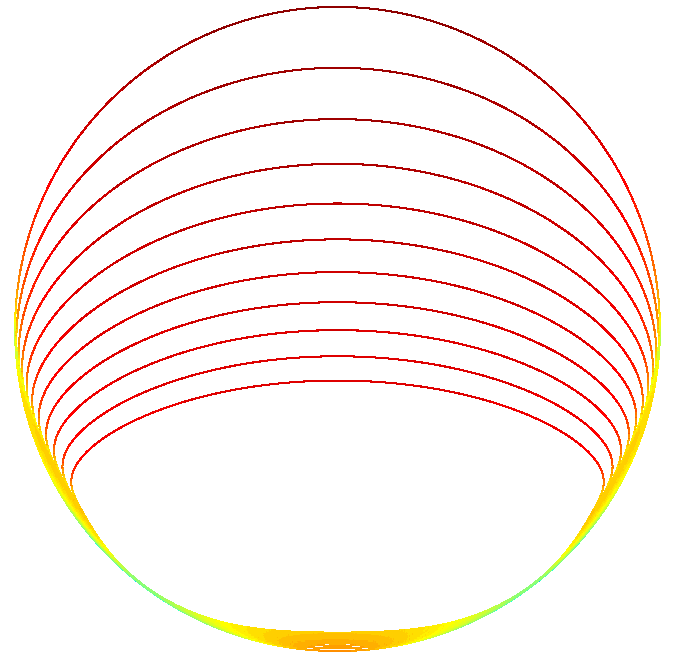
\includegraphics[height = 0.74\textwidth]{./figs/1b_0d4r1h_shear}
\caption{}
\end{subfigure}
\begin{subfigure}[b]{0.32\textwidth}
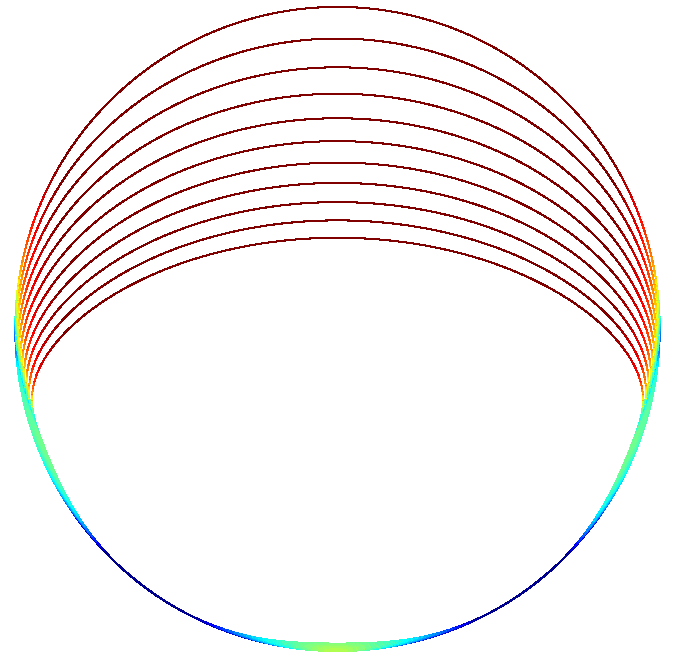
\includegraphics[height = 0.74\textwidth]{./figs/1b_0d4r0d5h_shear}
\caption{}
\end{subfigure}
\begin{subfigure}[b]{0.32\textwidth}
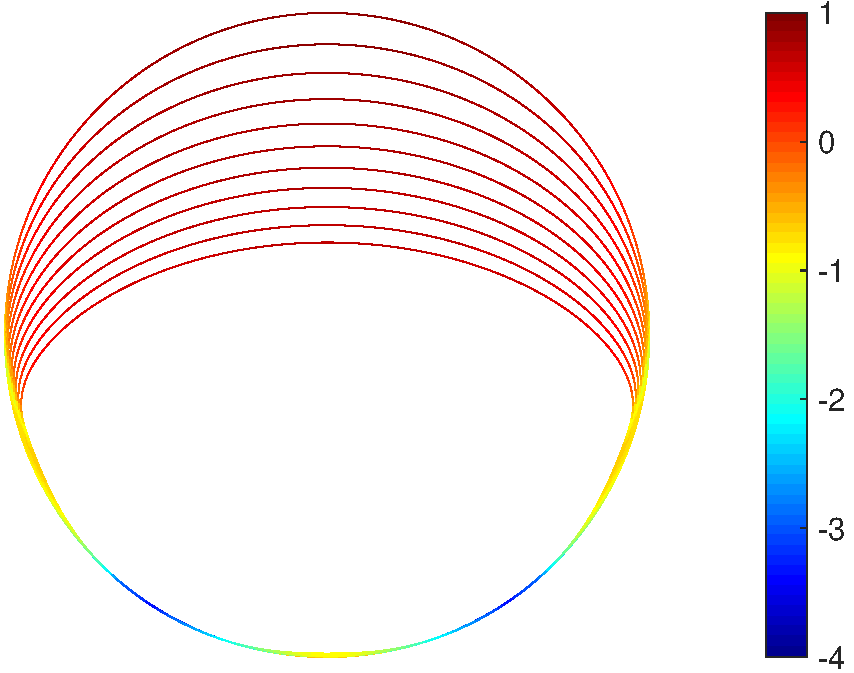
\includegraphics[height = 0.74\textwidth]{./figs/1b_0d4r0d1h_shear}
\caption{}
\end{subfigure}
\end{center}
\caption{\label{fig:NearWall} A single body eroding in a shearing Stokes
flow.  The color is the logarithm of the shear stress. Therefore,
erosion is fastest in the red regions (upper half) and slowest in the
blue regions (lower half).  The body is initialized at three different
distances from the lower wall: (a) $h$, (b) $h/2$, and (c) $h/10$.}
\end{figure}
\begin{figure}
\begin{center}
\begin{subfigure}[b]{0.32\textwidth}
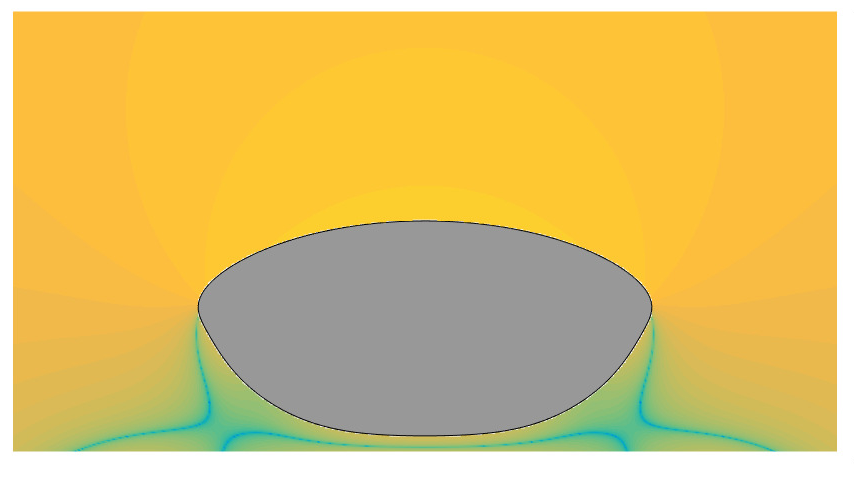
\includegraphics[height = 0.53\textwidth]{./figs/1b_0d4r1h_vort}
\caption{}
\end{subfigure}
\begin{subfigure}[b]{0.32\textwidth}
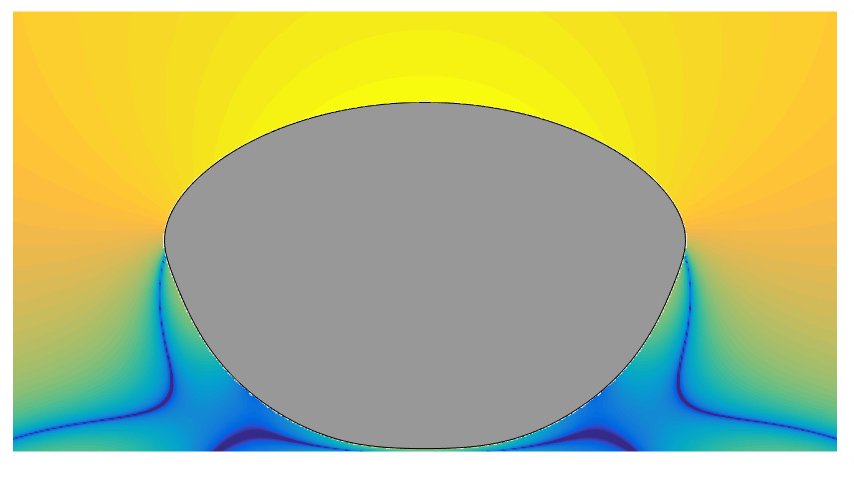
\includegraphics[height = 0.53\textwidth]{./figs/1b_0d4r0d5h_vort}
\caption{}
\end{subfigure}
\begin{subfigure}[b]{0.32\textwidth}
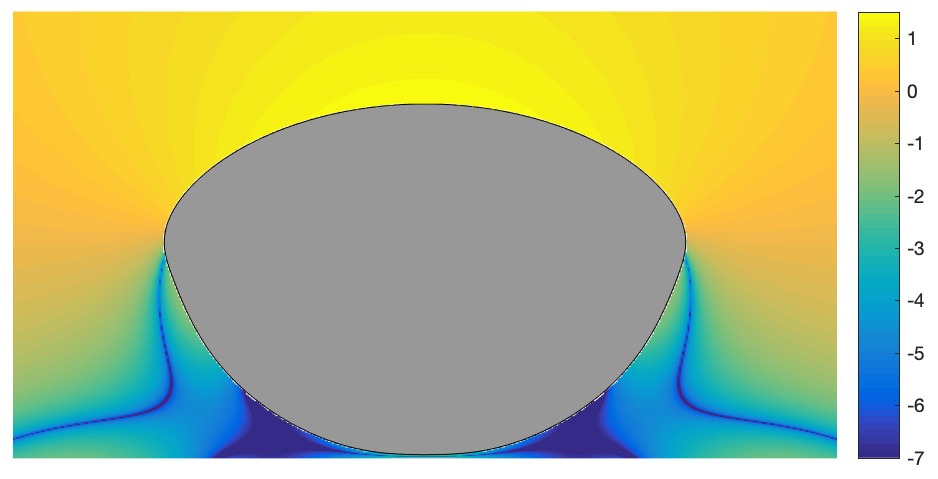
\includegraphics[height = 0.53\textwidth]{./figs/1b_0d4r0d1h_vort}
\caption{}
\end{subfigure}
\caption{\label{fig:NearWall_vort} The vorticity of the fluid with a
single body eroding at time $t=0.1$. The initial distance from the body
to the solid wall are: (a) $h$, (b) $h/2$, and (c) $h/10$.}
\end{center}
\end{figure}


%%%%%%%%%%%%%%%%%%%%%%%%%%%%%%%%%%%%%%%%%%%%%%%%%%%%%%%%%%%%%%%%%%%%%%%
\subsection{20 Bodies at a Medium Porosity}
\label{sec:Eroding20}
%%%%%%%%%%%%%%%%%%%%%%%%%%%%%%%%%%%%%%%%%%%%%%%%%%%%%%%%%%%%%%%%%%%%%%%
We consider 20 eroding grains with the Hagen-Poiseuille flow
\begin{align}
  \UU(\xx)=U \left[
  \begin{array}{c}
    1-y^2 \\ 0
  \end{array}
  \right],
\end{align}
imposed on $\Gamma$. The flow rate $U$ is chosen so that the average
pressure drop from $x=-2$ to $x=2$ is held fixed at 8. Therefore, $U=1$
once all the grains have vanished.  The vorticity and grain
configuration at four equispaced times are shown in
figure~\ref{fig:Eroding20vort}.  Initially, several of the grains are
closer to the outer wall than the $5h$ threshold required for the
trapezoid rule to achieve machine precision.  In particular, the
distance between bodies 1, 6, 13, and 15 and the outer wall is $1.3h$,
$2.9h$, $2.8h$, and $1.3h$, respectively, where $h$ is the arclength
spacing of the outer wall $\Gamma$.  In addition, the distance between
several pairs of eroding bodies, including 1 \& 6, 3 \& 9, 6 \& 8, and
14 \& 18, is too small to be accurately resolved with the trapezoid
rule.  By using the Barycentric quadrature rule, the interaction between
these nearly-touching bodies is accurately resolved to the desired
accuracy, and erosion can be simulated until all the bodies have
vanished.

\begin{figure}
\begin{center}
  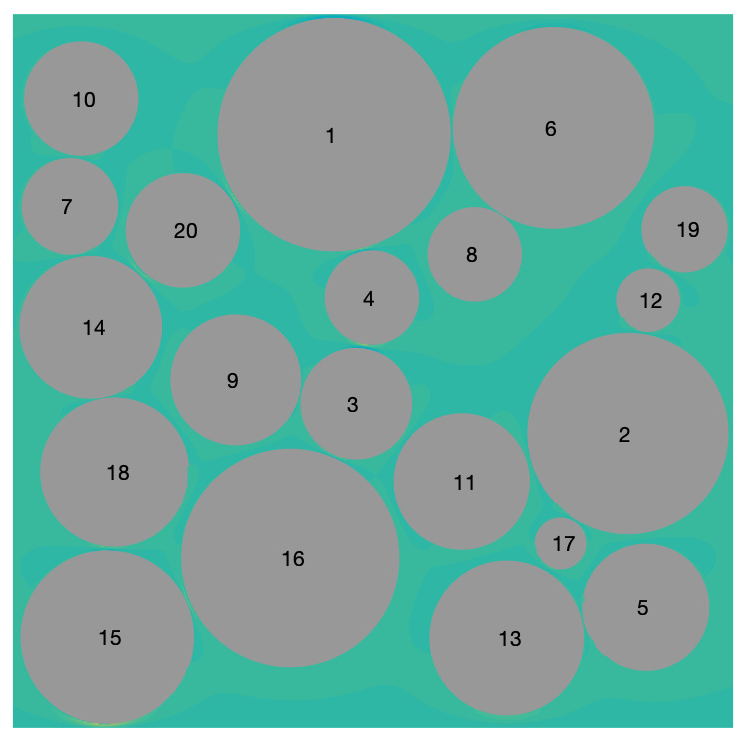
\includegraphics[height=0.227\textwidth]{./figs/20b_dense1}
  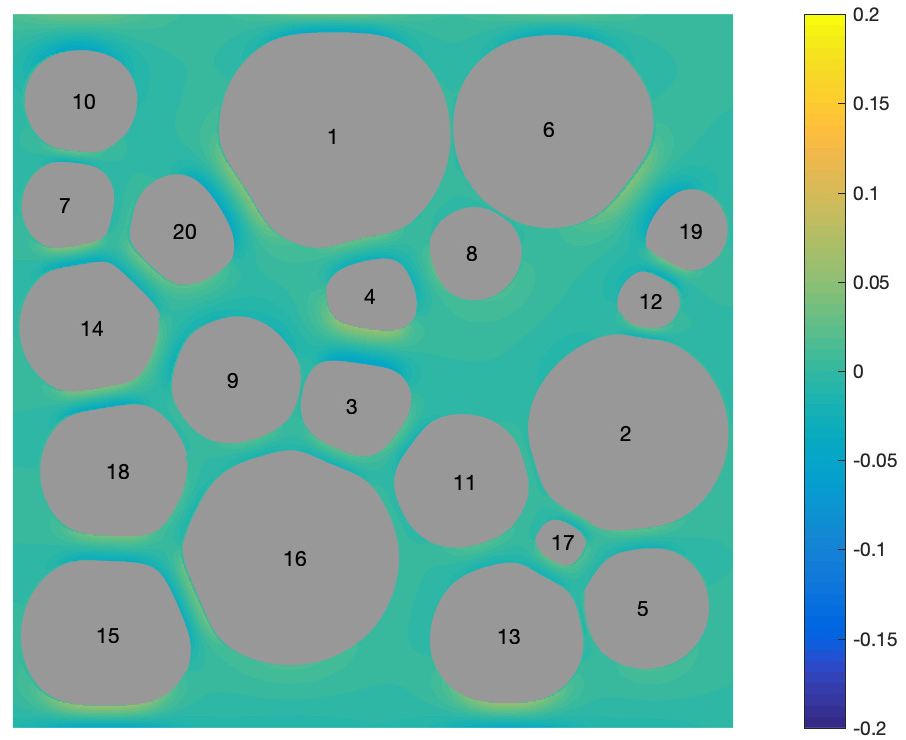
\includegraphics[height=0.227\textwidth]{./figs/20b_dense101}
  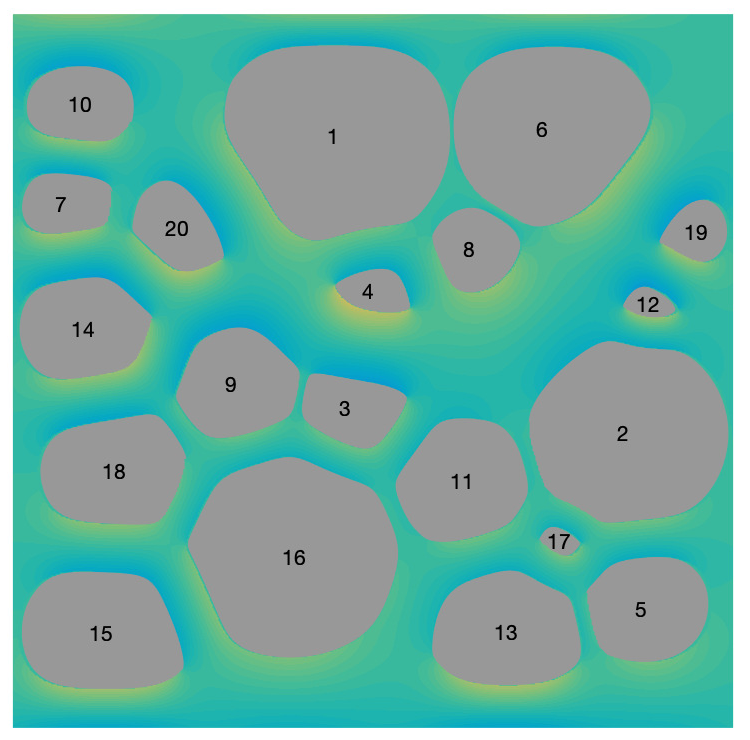
\includegraphics[height=0.227\textwidth]{./figs/20b_dense201}
  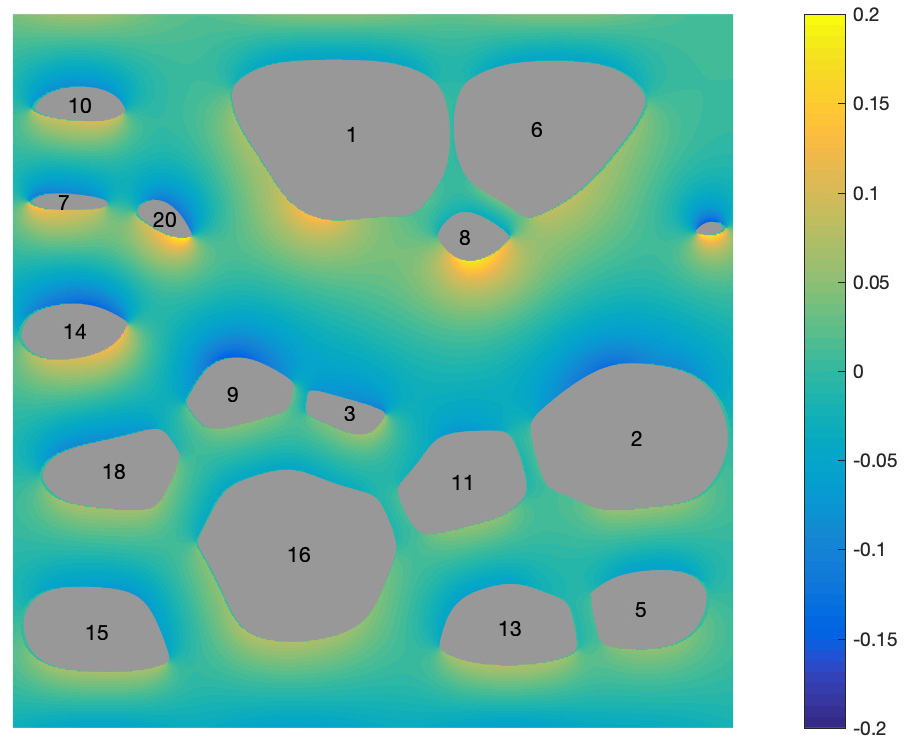
\includegraphics[height=0.227\textwidth]{./figs/20b_dense301}
\caption{\label{fig:Eroding20vort} The erosion of 20 nearly touching
bodies in a Hagen-Poiseuille flow.  The four snapshots are evenly spaced
in time, and the color is the fluid vorticity. In the fourth frame,
bodies 4, 12, and 17 have completely vanished, and body 19 has almost
completely eroded.}
\end{center}
\end{figure}

Erosion causes the some of the pore sizes to quickly grow, and flat
faces develop along the regions of near contact.  This qualitative
behavior is seen in figure~\ref{fig:Eroding20vort} between bodies 3 \&
4, 15 \& 16, and was also observed in previous work~\citep{qua-moo2018}.
However, by resolving the interaction between bodies that are much
closer together, we observe that very little erosion occurs between
certain pairs of bodies, at least initially.  For instance the opening
between bodies 1 \& 6, 3 \& 9, and 5 \& 13 grow much slower than the
opening between bodies 15 \& 16.  A common feature of the pores that
grow slowly is that they are nearly perpendicular to the main flow
direction, resulting in a small erosion rate.

\begin{figure}
\begin{subfigure}[b]{0.5\textwidth}
\includegraphics*[height = 0.7\linewidth]{./figs/porosity20dense}
\caption{}
\end{subfigure}
\begin{subfigure}[b]{0.5\textwidth}
\includegraphics*[height = 0.7\linewidth]{./figs/flow_rate20densen}
\caption{}
\end{subfigure}
\caption{\label{fig:Eroding20flowrate}(a) The area fraction of 20
nearly touching eroding bodies versus normalized time. (b) The flow
rate, $U$, for a fixed pressure drop across the channel versus
normalized time.  The flow rate is initially very small, but it
eventually increases as an exponential law  (dashed line) towards the
flow rate $U=1$ that occurs once all the bodies have eroded.}
\end{figure}

We next analyze the effect of erosion on the area fraction and the flow
rate.  In figure~\ref{fig:Eroding20flowrate}(a), we plot the area
fraction as a function of normalized time.  The general trend of the
area fraction resembles our previous work~\citep[see][figure
10(a)]{qua-moo2018}, but with a larger initial area fraction.  In
figure~\ref{fig:Eroding20flowrate}(b), we plot the flow rate $U$
required to maintain a constant pressure drop across the channel.
Again, the trend of $U$ resembles that of our previous
work~\citep[see][figure 10(b)]{qua-moo2018}, except that the initial
flow rate is an order of magnitude smaller because of the larger initial
area fraction.  Starting around normalized time $0.2$,
figure~\ref{fig:Eroding20flowrate}(b) is roughly linear which indicates
that the flow rate can be written as an exponential law.  The line of
best fit is
\begin{align}
  U \approx \exp\left(9.94 \left(\frac{t - t_f}{t_f} \right)\right),
\end{align}
which is the dashed line in figure~\ref{fig:Eroding20flowrate}(b).

\begin{figure}
\begin{center}
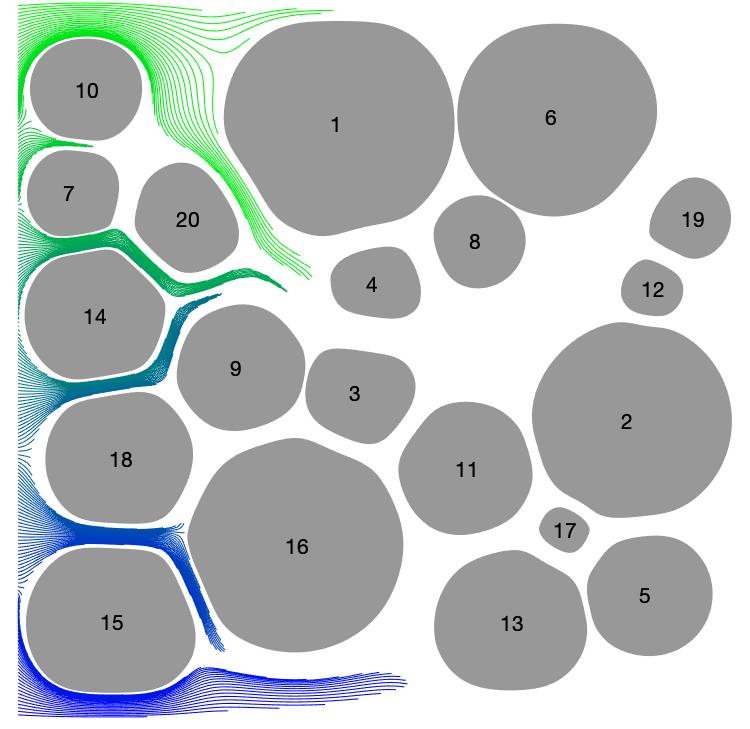
\includegraphics[width = 0.32 \textwidth]{./figs/tracer_20b30n}
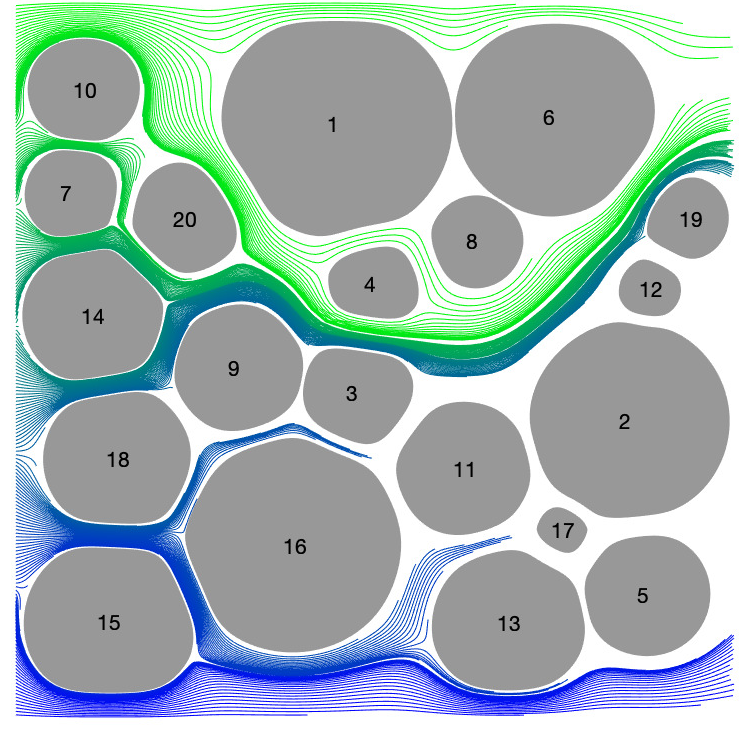
\includegraphics[width = 0.32 \textwidth]{./figs/tracer_20b90n}
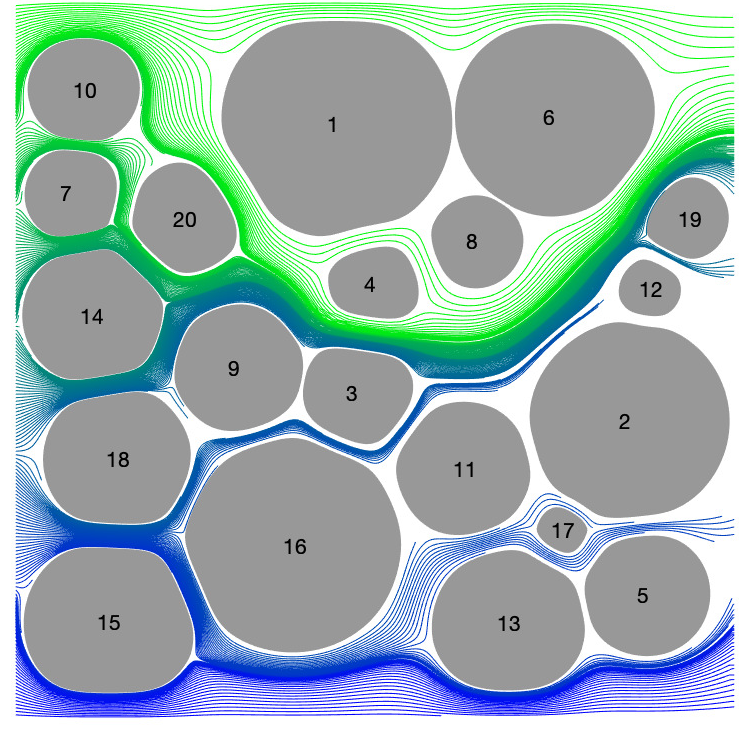
\includegraphics[width = 0.32 \textwidth]{./figs/tracer_20b150n}\\
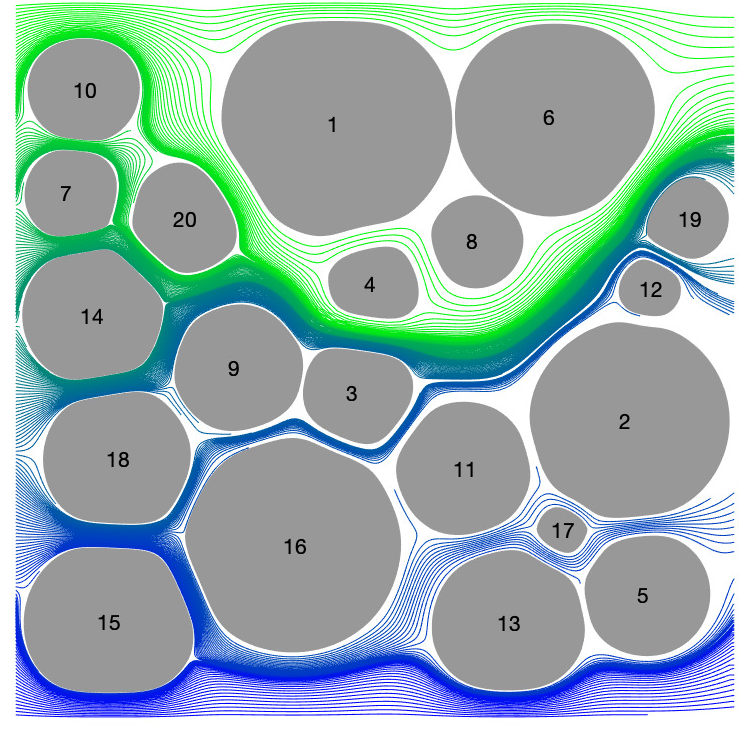
\includegraphics[width = 0.32 \textwidth]{./figs/tracer_20b210n}
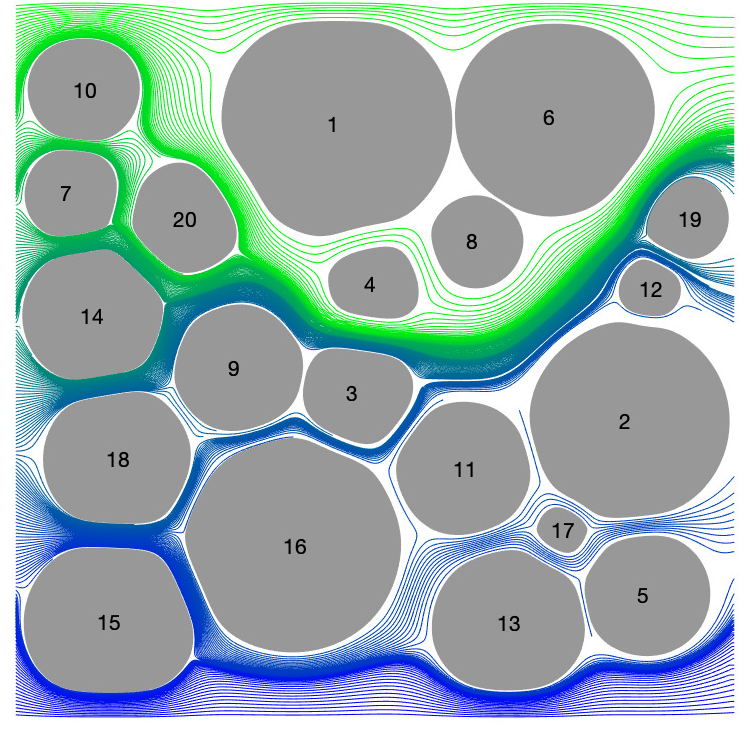
\includegraphics[width = 0.32 \textwidth]{./figs/tracer_20b270n}
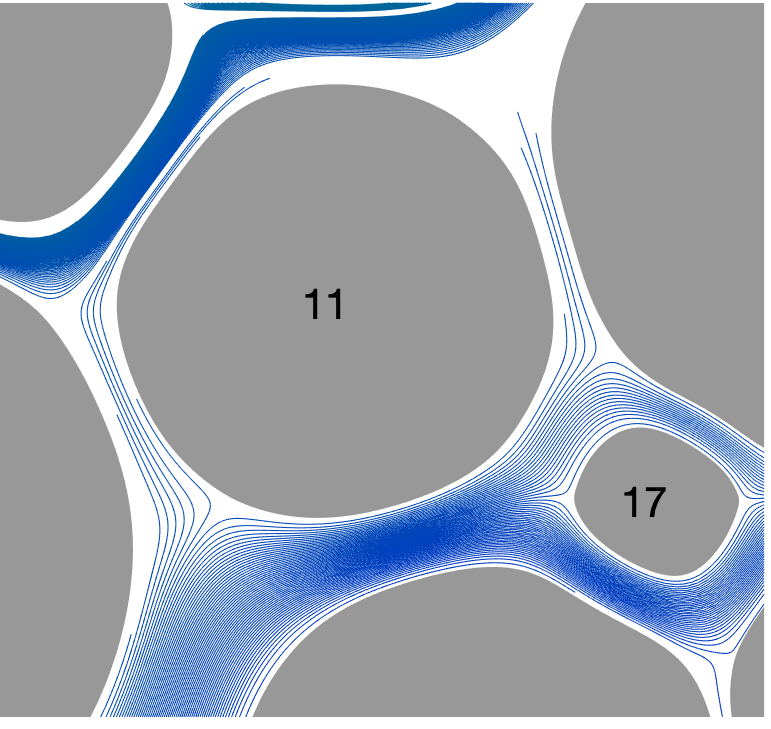
\includegraphics[width = 0.32 \textwidth]{./figs/tracer_20b270n_zoom}
\caption{\label{fig:Eroding20tracer} 200 streamlines in the second
geometry from figure~\ref{fig:Eroding20vort}. The streamlines are
initially equispaced at $(-1,y)$, where $y \in (-1,1)$. The first five
snapshots are evenly spaced in time.  The bottom right frame is a zoom
in of the fifth snapshot, but with additional streamlines.  Since we use
the Barycentric quadrature rule and a fourth-order Runge-Kutta method,
streamlines that are very close to the grains are resolved.}
\end{center}
\end{figure}


In figure~\ref{fig:Eroding20vort}, we observe that erosion creates a
network of channels from the inlet to the outlet where the velocity and
vorticity, and therefore erosion rate, are much larger relative to other
regions.  These channels can be further visualized  with the
streamlines.  In figure~\ref{fig:Eroding20tracer}, we freeze the
geometry at the second snapshot from figure~\ref{fig:Eroding20vort} and
plot 200 streamlines that are initially equispaced along $(-1,y)$, where
$y \in (-1,1)$.  The streamlines are shown at five different times, and
the final plot is a zoom in of the lower right quadrant of the fifth
time step, but with additional streamlines.  Since we use a high-order
quadrature rule and time stepping method, we resolve streamlines that
come very close to the eroded bodies.  There are three clear regions
where the streamlines are most concentrated, corresponding to the
regions of highest velocity.  Two of these regions are located between
the bodies and the solid walls at $y=\pm 1$, and the third cuts through
the porous region with the upper part of the channel formed by bodies 1,
4, 6, and 8.  Since the flow is fastest in these regions, the shearing
is largest, and this causes the channels to continue to open fastest as
observed in figure~\ref{fig:Eroding20vort}.

Next, we use the $N_p = 1000$~\citep{bel-sal-rin1992} streamlines to
compute the tortuosity of the eroding geometry.  To compute the
tortuosity, we require the velocity at the inlet $x=-1$.  These
normalized velocities are plotted in figure~\ref{fig:Eroding20tort}(a)
for the eroded geometry at porosity $\phi = 62.9\%$
(figure~\ref{fig:Eroding20tort}(c)).  The velocities are similar those
of~\citet[see figure 4(a)]{mat-kha-koz2008}, except that our
cross-section, by construction, does not cut through any of the grains.
Next, in figure~\ref{fig:Eroding20tort}(b), we plot the local
tortuosity~\eqref{eqn:localTort} by calculating the relative length of
each streamline as it traverses the channel from $x=-1$ to $x=1$.  The
local tortuosity ranges from 1 to 1.27, meaning that one of the
streamlines is 27\% longer than it would have been if the grains were
absent.  The average streamline is 9.79\% longer or equivalently the
tortuosity of the geometry is $1.098$.  Again, comparing the local
tortuosity to~\citet[see figure 4(b)]{mat-kha-koz2008}, the results are
qualitatively similar. However, since our initial cross-section does not
cut through the grains, the local tortuosity does not have any gaps.
Discontinuities in local tortuosity occur when nearby streamlines
diverge to circumvent a grain.  In figure~\ref{fig:Eroding20tort}(c), we
plot pairs of streamlines associated with the ten largest jumps in the
local tortuosity, with each pair of corresponding streamlines plotted in
the same color.

\begin{figure}
\begin{subfigure}[b]{0.45\textwidth}
\begin{subfigure}[b]{\textwidth}
\includegraphics*[width =\linewidth]{./figs/velocity_loc20_268}
\caption{}
\end{subfigure}
\begin{subfigure}[b]{\textwidth}
\includegraphics*[width =0.97\linewidth]{./figs/tort_local20_268}
\caption{}
\end{subfigure}
\end{subfigure}
\begin{subfigure}[b]{0.5\textwidth}
\includegraphics*[width =\linewidth]{./figs/tort_diff_top10_268}
\caption{}
\end{subfigure}
\caption{\label{fig:Eroding20tort} The tortuosity of a porous geometry
that initially had 20 grains and has eroded to a porosity of 62.9\%.
(a) The $x$-component of the velocity at the inlet, $u_1(-1,y)$,
normalized by its maximum velocity of $2.98 \times 10^{-3}$. (b) The
local tortuosity $\tau(y)$ on the cross section $x = -1$.  The spatially
averaged tortuosity through the channel is $1.098$.  (c) The streamlines
resulting in the ten largest differences of local tortuosity between
neighboring streamlines.  Neighboring streamlines have the same color.}
\end{figure}

In figure~\ref{fig:Eroding20Transport}(a), we plot the tortuosity as a
function of the porosity. The initial porosity is $\phi = 37.68\%$, and
the initial tortuosity is $T = 1.16$.  The tortuosity is computed with
both the length of the streamlines~\eqref{eqn:tortuosity1} (red stars)
and using the spatial average of the velocity on an Eulerian
grid~\eqref{eqn:tortuosity2} (blue marks).  The red square corresponds
to the porosity of the geometry in figure~\ref{fig:Eroding20tort}(c).
The two tortuosity formulas give similar results, and any discrepancy
can be accounted for by slow regions of recirculation and from applying
quadrature to compute the tortuosity.  As the bodies erode, wide
channels form where streamlines undergo only minor vertical deflections,
and this explains why the tortuosity eventually decreases with porosity.
We computed lines of best fit using the porosity-tortuosity
models~\eqref{eqn:tortuosityModels} and found that the power law
minimizes the error.  The  black dashed line in
figure~\ref{fig:Eroding20Transport}(a) is the line of best fit
\begin{align}
  \widehat{T}(\phi) = \phi^{-0.2064},
\end{align}
with a root-mean-square error of $5.90 \times 10^{-3}$.  Interestingly,
at the low porosities, the tortuosity initially increases. This increase
occurs because in the absence of erosion (left plot in
figure~\ref{fig:Eroding20vort}), many of the streamlines, such as those
initialized between bodies 15 \& 18, only perform minor deflections to
pass through the narrow regions, albeit, very slowly.  However, as
erosion starts to open the channels, the streamlines deflect into the
fast regions, such as the region above body 11, and this increases the
amount of vertical deflection, and therefore the tortuosity. While this
increase in tortuosity is interesting, in the next two examples we will
see that the tortuosity does not initially increase.

We next use streamlines to investigate the temporal evolution of the
particle spreading $\sigma_\lambda$.  The spreading is computed for
seven geometries of different porosities that are formed during the
erosion process (figure~\ref{fig:Eroding20Transport}(b)).  So that the
spreading reaches a statistical equilibrium, we use the reinsertion
algorithm described in section~\ref{sec:dispersion} to form sufficiently
long trajectories.  For all the reported porosities, the particle
dispersion exhibits two distinct power law regimes.  Initially, the
dispersion is ballistic ($\sigma_\lambda \sim t$) since individual fluid
particles have not yet explored enough space to significantly alter
their velocity.  However, once the particles have been subjected to a
range of velocities, their dispersion slows, and we observe
super-dispersive ($\sigma_\lambda \sim t^\alpha$, $\alpha \in (1/2,1)$)
behavior over at least one order of magnitude in time.  Before any
erosion takes place, the anomalous dispersion coefficient is $\alpha =
0.56$.  Then, as the grains begin to erode, the dispersion rate grows
towards the ballistic regime that occurs in the absence of grains.  The
monotonic increase in dispersion with respect to the porosity is
explained by the onset of channels where many tracers experience less
variability in their velocities.

\begin{figure}
\begin{subfigure}[b]{0.5\textwidth}
\includegraphics*[height = 0.8\linewidth]{./figs/tort_eulerian}
\caption{}
\end{subfigure}
\begin{subfigure}[b]{0.5\textwidth}
\includegraphics*[height = 0.8\linewidth]{./figs/20b_second_moment_long_ref}
\caption{}
\end{subfigure}
\caption{\label{fig:Eroding20Transport} (a) The tortuosity of an eroding
geometry initialized with 20 grains.  The tortuosity is calculated using
the Eulerian method~\eqref{eqn:tortuosity2} (blue dots) and Lagrangian
method~\eqref{eqn:tortuosity1} (red stars).  The red square corresponds
to the geometry in figure~\ref{fig:Eroding20tort}(c).  The dash line is
the line of best fit $\widehat{T}(\phi)=\phi^{-p}$ with $p=0.2064$, and
the corresponding root-mean-square error is $5.90 \times 10^{-3}$. (b)
The temporal evolution of $\sigma_\lambda$ as a function of time at
seven different porosities.  The dashed line, which has slope one,
corresponds to ballistic dispersion $\sigma_\lambda \sim t$ that occurs
if no grains are present. At early times, the particles undergo a
ballistic motion, but once they have traversed a few grains, the
spreading becomes super-dispersive with $\sigma_\lambda \sim t^\alpha$,
$\alpha \in (1/2,1)$.  The dashed-dotted lines are lines of best fit
with slopes $\alpha = 1.06$ ($\phi=95.10\%$), $\alpha = 1.07$
($\phi=85.09\%$), $\alpha = 1.06$ ($\phi=75.15\%$), $\alpha = 0.97$
($\phi=65.09\%$), $\alpha = 0.78$ ($\phi=55.10\%$), $\alpha = 0.75$
($\phi=45.08\%$), and $\alpha = 0.56$ ($\phi=37.68\%$).  Values greater
than 1 result from using a least-squares fit for the tails of the
particle spreading.}
\end{figure}


%%%%%%%%%%%%%%%%%%%%%%%%%%%%%%%%%%%%%%%%%%%%%%%%%%%%%%%%%%%%%%%%%%%%%%%
\subsection{20 Bodies at a Low Porosity}
%%%%%%%%%%%%%%%%%%%%%%%%%%%%%%%%%%%%%%%%%%%%%%%%%%%%%%%%%%%%%%%%%%%%%%%
We consider a second example with 20 eroding bodies, but with a smaller
initial porosity.  In figure~\ref{fig:ErodingLow20vort}, we plot the
eroding geometry and vorticity at four evenly spaced instances in time.
Initially, the smallest distance between pairs of bodies is $3.29 \times
10^{-4}$, and the smallest distance between the bodies and solid wall is
$4.50 \times 10^{-3}$.  At these distances, a resolution of
approximately $N_\iin = 27,000$ and $N_\out = 18,000$ discretization
points is required to satisfy the $5h$ threshold needed for the
trapezoid rule to achieve machine precision.

\begin{figure}
\begin{center}
  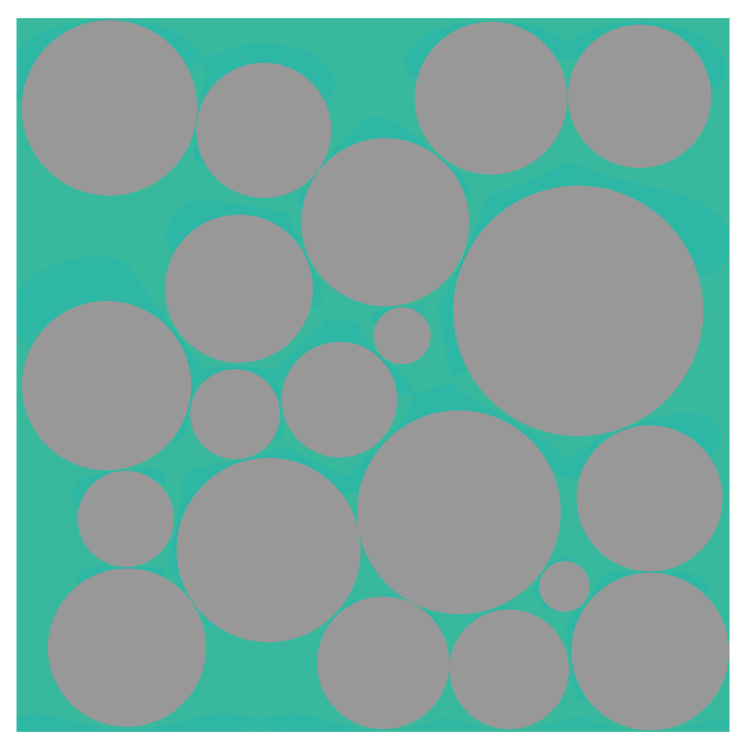
\includegraphics[height=0.227\textwidth]{./figs/20b2_vort1}
  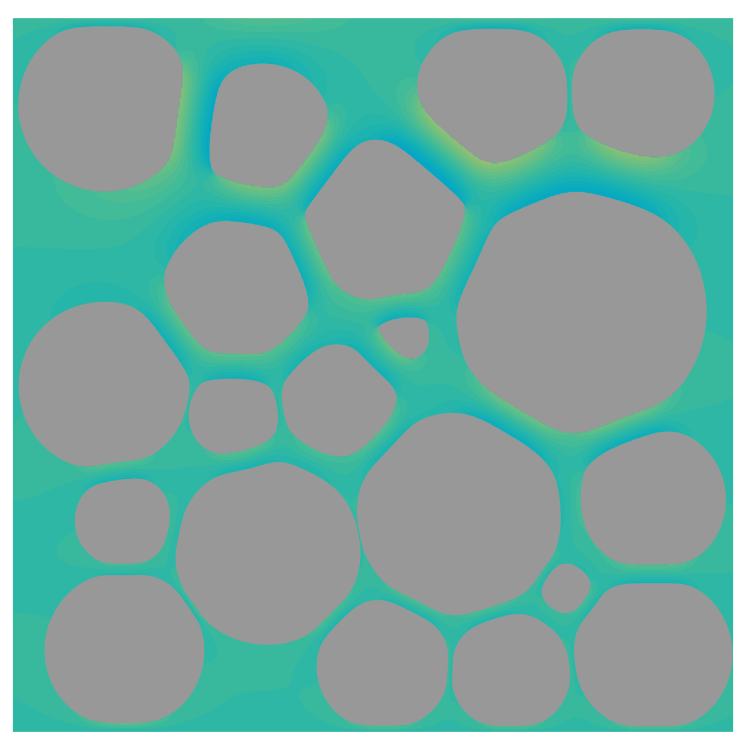
\includegraphics[height=0.227\textwidth]{./figs/20b2_vort150}
  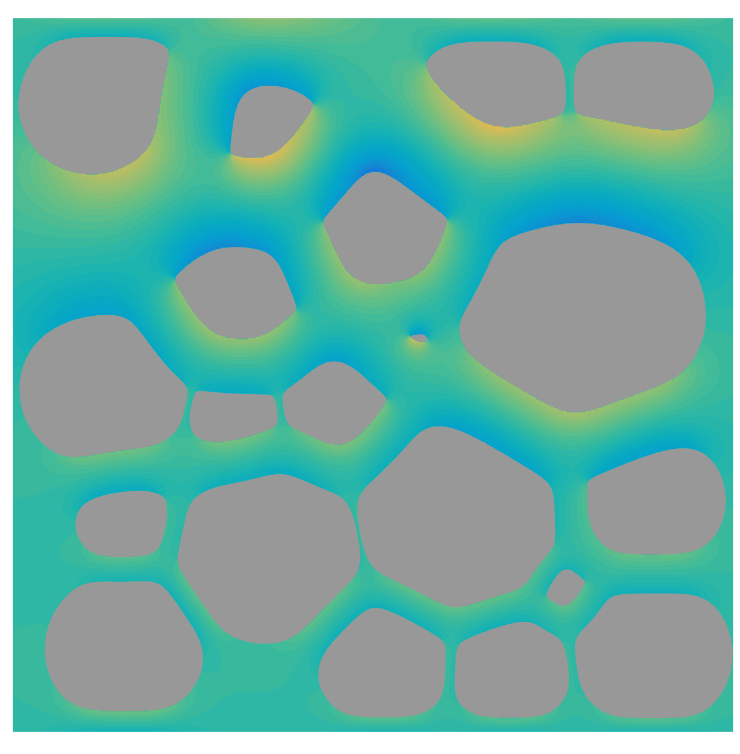
\includegraphics[height=0.227\textwidth]{./figs/20b2_vort300}
  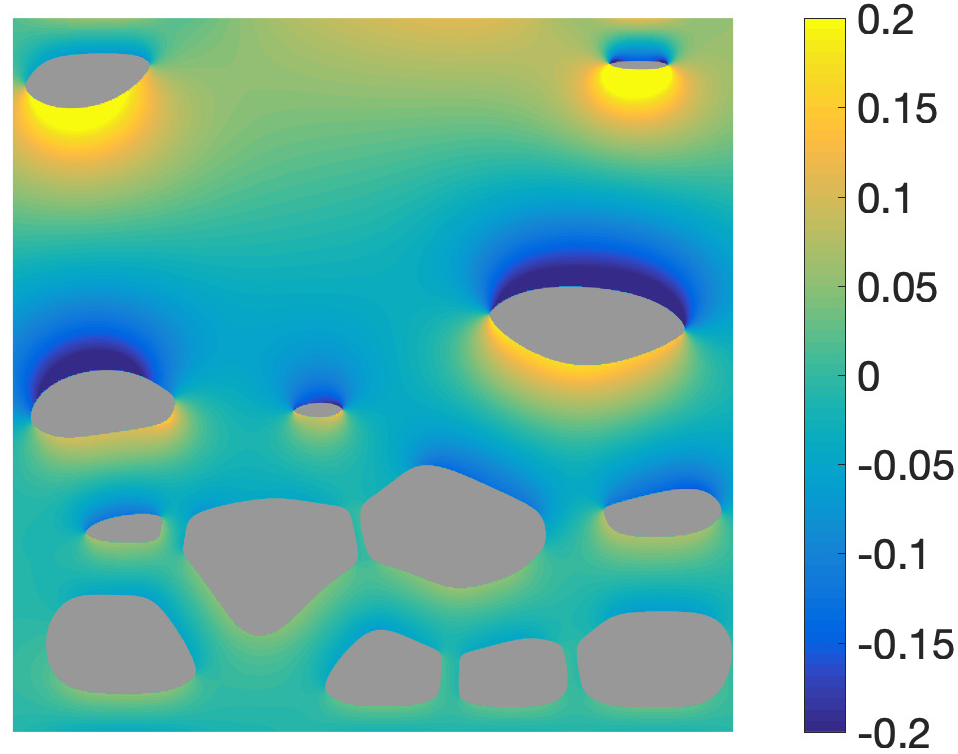
\includegraphics[height=0.227\textwidth]{./figs/20b2_vort450}
\end{center}
\caption{\label{fig:ErodingLow20vort} The erosion of 20 nearly touching
bodies in a Hagen-Poiseuille flow. The four snapshots are evenly spaced
in time, and the color is the fluid vorticity. In addition to the
channels that develop between the bodies and the solid walls, erosion
leads to two main channels through the geometry---one in the top half
and one near the middle.}
\end{figure}

We compute the tortuosity using the Eulerian
method~\eqref{eqn:tortuosity2} at each time step. The initial porosity
is $\phi = 30.67\%$ and the initial tortuosity is $T = 1.24$.  In
figure~\ref{fig:ErodingLow20Transport}(a), we plot the tortuosity with
respect to the porosity (blue) and the line of best fit (black) using
the power law 
\begin{align}
  \widehat{T}(\phi) = \phi^{-0.1669}.
\end{align}
This model outperforms the other three models in
equation~\eqref{eqn:tortuosityModels}, and its root-mean-squared error
is $1.13 \times 10^{-2}$.  As grains erode, there is an increase in the
number of streamlines that take a nearly direct path through the
geometry, and this decreases the tortuosity. However, the channelization
effect of erosion results in an increase in the tortuosity since the
length of many of the streamlines increases when they deflect from a
high porosity region (low pressure) to a low porosity region (high
pressure). For this example, we see that the net effect is a decrease in
the tortuosity for all time.

\begin{figure}
\begin{subfigure}[b]{0.5\textwidth}
\includegraphics*[height = 0.8\linewidth]{./figs/tort_eulerian20b}
\caption{}
\end{subfigure}
\begin{subfigure}[b]{0.5\textwidth}
\includegraphics*[height=0.8\linewidth]{./figs/20b_dense_second_moment_ref}
\caption{}
\end{subfigure}
\caption{\label{fig:ErodingLow20Transport} (a) The tortuosity of an
eroding geometry initialized with 20 grains.  When compared to the last
example, the bodies are initially much closer together, and the porosity
is smaller.  The tortuosity is calculated with the Eulerian
method~\eqref{eqn:tortuosity2} (blue dots).  The dash line is the
fitting line $\widehat{T}(\phi)=\phi^{-p}$ with $p=0.1669$, and the root
mean square deviation is $1.13 \times 10^{-2}$.  (b) The temporal
evolution of $\sigma_\lambda$ as a function of time at eight different
porosities.  The dashed line, which has slope one, corresponds to
ballistic dispersion $\sigma_\lambda \sim t$ that occurs if no grains
are present.  At early times, the particles undergo a ballistic motion,
but once they have traversed a few grains, the spreading becomes
super-dispersive with $\sigma_\lambda \sim t^{\alpha}$, $\alpha \in
(1/2,1)$.  The dashed-dotted lines are lines of best fit with slope
$0.92$ ($\phi=95.00\%$), $0.87$ ($\phi=85.17\%$), $0.87$
($\phi=75.10\%$), $0.91$ ($\phi=65.02\%$), $0.91$ ($\phi=55.08\%$),
$0.72$ ($\phi=45.03\%$), $0.69$ ($\phi=35.05\%$), and $0.92$
($\phi=30.67\%$).}
\end{figure}

In figure~\ref{fig:ErodingLow20Transport}(b), we plot the temporal
evolution of the particle spreading $\sigma_\lambda$.  As in the last
example, we analyze the spreading at several different porosities and we
use the reinsertion algorithm described in section~\ref{sec:dispersion}.
For all the porosities, the dispersion is much closer to ballistic when
compared to the results in figure~\ref{fig:Eroding20Transport}.
However, there are still clear transitions from ballistic dynamics to
asymptotic super-dispersive spreading.  In contrast to the higher
porosity initial condition (section~\ref{sec:Eroding20}), at early times
the erosion results in a decrease in the dispersion rate. In particular,
after the first 5\% of the bodies have eroded, the particle spreading
transitions from $\sigma_\lambda \sim t^{0.92}$ to $\sigma_\lambda \sim
t^{0.69}$.  To explain this behavior, recall that anomalous dispersion
is caused by tracers spending time in both the fast and slow regimes.
Since the initial configuration has a reasonably uniform velocity (see
figure~\ref{fig:ErodingLow20vort}), albeit a small one, the dispersion
is nearly ballistic. However, as the geometry erodes, the flow becomes
more intermittent, and this results in an increased anomalous dispersion
rate~\citep{dea-leb-den-tar-bol-dav2013}.  Then, as the bodies continue
to erode, the geometry channelizes, and most tracers are transported
with a large velocity through the channels, again resulting in a nearly
ballistic motion~\citep{sie-ili-pri-riv-gua2019}.

%%%%%%%%%%%%%%%%%%%%%%%%%%%%%%%%%%%%%%%%%%%%%%%%%%%%%%%%%%%%%%%%%%%%%%%
\subsection{100 eroding bodies}
\label{sec:Eroding100}
%%%%%%%%%%%%%%%%%%%%%%%%%%%%%%%%%%%%%%%%%%%%%%%%%%%%%%%%%%%%%%%%%%%%%%%
As a final example, we consider 100 eroding bodies with an initial
porosity near 50\%.  Snapshots of the configurations and vorticity are
in figure~\ref{fig:Eroding100vort}. We compute the tortuosity using both
the Lagrangian~\eqref{eqn:tortuosity1} and Eulerian
methods~\eqref{eqn:tortuosity2}. Therefore, we compute and plot the
normalized velocity
at $N_p = 1000$ points along the inlet $x=-1$ in figure~\ref{fig:Eroding100tort}(a) for the
eroded geometry at porosity $\phi = 62.98\%$
(figure~\ref{fig:Eroding100tort}(c)).  The initial velocity of the
tracers is qualitatively similar to the 20 body example
(figure~\ref{fig:Eroding20tort}(a)), except with additional oscillations
because of the additional grains.  In
figure~\ref{fig:Eroding100tort}(b), we plot the local tortuosity by
finding the length of the streamlines as they pass from $x=-1$ to $x=1$.
Compared to figure~\ref{fig:Eroding20tort}(b), the local tortuosity is
much more discontinuous.  These discontinuities can be explained by
examining the trajectories of tracers in
figure~\ref{fig:Eroding100tort}(c).  Here, there are many instances of
nearby streamlines that are deflected apart from one another as they
tend to a stagnation point in the flow, and this results in trajectories
with significantly different lengths.  At this porosity, one of the
tracers travels 25.5\% farther than it would have if the bodies had been
absent, and the average tracer travelled 12\% farther resulting in a
tortuosity of $T = 1.12$.

\begin{figure}
\begin{subfigure}[b]{0.5\textwidth}
\includegraphics*[height =0.8\linewidth]{./figs/100b_50}
\caption{100 bodies, $\phi = 55.54\%$}
\end{subfigure}%
\begin{subfigure}[b]{0.5\textwidth}
\includegraphics*[height =0.8\linewidth]{./figs/100b_100}
\caption{99 bodies, $\phi = 62.98\%$}
\end{subfigure}
\begin{subfigure}[b]{0.5\textwidth}
\includegraphics*[height =0.8\linewidth]{./figs/100b_150}
\caption{94 bodies, $\phi = 72.22\%$}
\end{subfigure}%
\begin{subfigure}[b]{0.5\textwidth}
\includegraphics*[height =0.8\linewidth]{./figs/100b_200}
\caption{82 bodies, $\phi = 83.67\%$}
\end{subfigure}
\caption{\label{fig:Eroding100vort} The erosion of 100 nearly touching
grains in a Hagen-Poiseuille flow. The four snapshots are evenly spaced
in time, and the color is the fluid vorticity.  Because of the large
number of bodies, erosion creates many channels connecting the inlet to
the outlet.}
\end{figure}

In figure~\ref{fig:Eroding100Transport}(a), we plot the tortuosity as a
function of the porosity.  The initial geometry has a porosity of $\phi
= 50.09\%$ and the tortuosity is $T = 1.20$.  The tortuosity is computed
with both the length of the streamlines~\eqref{eqn:tortuosity1} (red
stars) and using the spatial average of the velocity on an Eulerian
grid~\eqref{eqn:tortuosity2} (blue marks).  The red square corresponds
to the porosity of the geometry in figure~\ref{fig:Eroding100tort}(c).
Again, the two tortuosity formulas give similar results.  For this
geometry, the tortuosity decreases monotonically at almost all
porosities.  However, the tortuosity undergoes a sudden increase near
the end of the simulation, and we have observed this behavior in other
examples.  The increase is caused by a single small body near the middle
of the channel being completely eroded.  While this results in
straighter streamlines, therefore reducing $\lambda$, the horizontal
flow, $u_1(y)$, increases since there is no longer a no-slip boundary,
and this increases the tortuosity.  We also compute the lines of best
fit using the porosity-tortuosity models~\eqref{eqn:tortuosityModels}.
The black dashed line in figure~\ref{fig:Eroding100Transport}(a) is the
line of best fit
\begin{align}
  \widehat{T}(\phi) = \phi^{-0.2459},
\end{align}
with a root-mean-square error of $5.50 \times 10^{-3}$.  We note a
slightly better root-mean-square error of $5.20 \times 10^{-3}$ is
possible with the model
\begin{align}
  \widehat{T}(\phi) = 1 - 0.2631 \ln(\phi).
\end{align}

\begin{figure}
\begin{subfigure}[b]{0.45\textwidth}
\begin{subfigure}[b]{\textwidth}
\includegraphics*[width =\linewidth]{./figs/velocity_loc100}
\caption{}
\end{subfigure}
\begin{subfigure}[b]{\textwidth}
\includegraphics*[width =\linewidth]{./figs/tort_local100}
\caption{}
\end{subfigure}
\end{subfigure}
\begin{subfigure}[b]{0.5\textwidth}
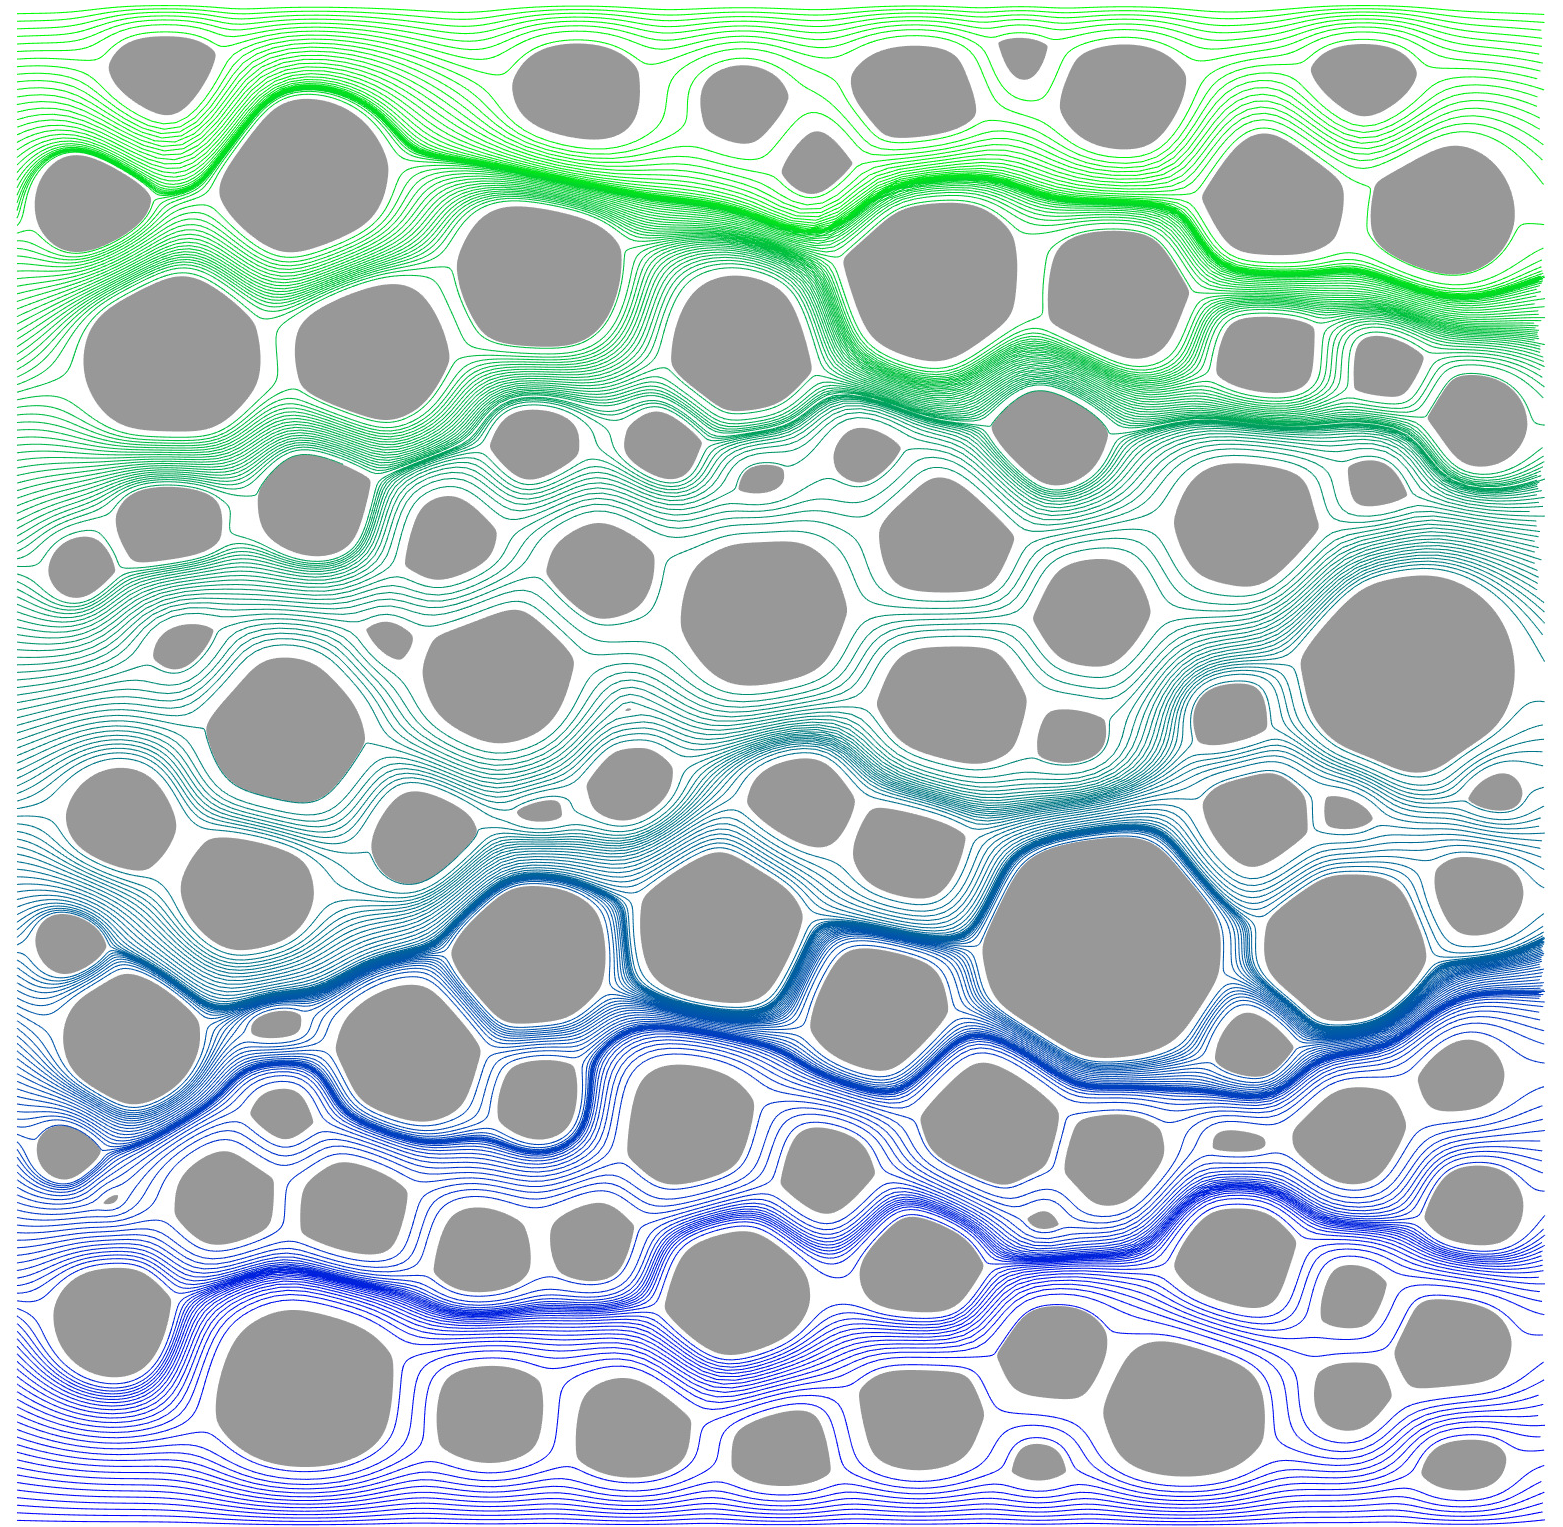
\includegraphics[width = \textwidth]{./figs/100b_t100tracer}
\caption{}
\end{subfigure}
\caption{\label{fig:Eroding100tort} The tortuosity of a porous geometry
that initially had 100 grains and has eroded to a porosity of 62.98\%.
(a) The $x$-component of the velocity at the inlet, $u_1(-1, y)$,
normalized by its maximum velocity $u_{max}=3.90 \times 10^{-4}$.  Note
that this maximum velocity is about a order of magnitude smaller than
the 20 body example in figure~\ref{fig:Eroding20tort}.  (b) The local
tortuosity $\tau(y)$ on the cross section $x = -1$. The spatially
averaged tortuosity through the channel is $T = 1.12$. (c) The
trajectories of 200 tracers initialized at $x = -1$.  The
discontinuities in the local tortuosity correspond to nearby streamlines
whose lengths are significantly different because they pass opposite
sides of an eroding body. Compared to figure~\ref{fig:Eroding20tort},
this example has more small bodies, and this results in many more
discontinuities.}
\end{figure}

In figure~\ref{fig:Eroding100Transport}(b), we plot the temporal
evolution of the particle spreading $\sigma_\lambda$ at six different
porosities. Again, we initially observe ballistic motion (black dashed
line), and then super-dispersion.  Similar to the example in
figure~\ref{fig:ErodingLow20Transport}(b), the asymptotic anomalous
dispersion rate is not growing with the porosity.  Therefore, it appears
that the dispersion rate in an eroding geometry depends not only the
porosity, but also the location and shape of the bodies.  Finally, at
the highest porosity, anomalous dispersion is only observed briefly in
the time interval $(0.5,1)$, and then transitions back to a ballistic
regime.  Since the bodies are so small at this high porosity, after
reinsertion, the streamline is not significantly deflected by any of the
bodies, and this results in a ballistic regime.

\begin{figure}
\begin{subfigure}[b]{0.5\textwidth}
\includegraphics*[height = 0.8\linewidth]{./figs/tort_eulerian100}
\caption{}
\end{subfigure}
\begin{subfigure}[b]{0.5\textwidth}
\includegraphics*[height=0.8\linewidth]{./figs/100b_second_moment_long_ref}
\caption{}
\end{subfigure}
\caption{\label{fig:Eroding100Transport} (a) The tortuosity of an
eroding geometry initialized with 100 grains.  The tortuosity is
calculated using the Eulerian method~\eqref{eqn:tortuosity2} (blue dots)
and Lagrangian method~\eqref{eqn:tortuosity1} (red stars).  The dash
line is the fitting line $\widehat{T}(\phi)=\phi^{-p}$ with $p=0.2459$,
and the root-mean-square error is $5.50 \times 10^{-3}$.  We note that
the model $\widehat{T}(\phi) = 1 - p \ln (\phi)$, with $p=0.2631$, has a
comparable root-mean-square error of $5.20 \times 10^{-3}$.  (b) The
temporal evolution of $\sigma_\lambda$ as a function of time at six
different porosities.  The dashed line, which has slope one, corresponds
to ballistic dispersion $\sigma_\lambda \sim t$ that occurs if no bodies
are present.  At early times, the particles undergo a ballistic motion,
but once they have traversed a few grains, the spreading becomes
super-dispersive with $\sigma_\lambda \sim t^{\alpha}$, $\alpha \in
(1/2,1)$.  The dashed-dotted lines are lines of best fit with slope
$1.11$ ($\phi=95.12\%$), $0.68$ ($\phi=85.07\%$), $0.73$
($\phi=75.14\%$), $0.59$ ($\phi=65.03\%$), $0.61$ ($\phi=55.02\%$), and
$0.70$ ($\phi=50.09\%$).}
\end{figure}

Finally, we investigate the effect of erosion on pore sizes.  The
distribution of the pore sizes is directly related to the
distribution of the velocity, and thus effects the
tortuosity~\citep{den-ica-hid2018} and anomalous
dispersion~\citep{dea-qua-bir-jua2018}. In addition, the pore sizes are
used in network models~\citep{bry-mel-cad1993, bry-kin-mel1993}.  As
described in section~\ref{sec:throats}, we use a Delaunay triangulation
to define neighboring eroding bodies, and we compute the pore size by
finding the closest distance between all neighboring bodies.  Instead of
computing a Delanuay configuration at each time step, which would result
in new definitions for the pores at each time step, we only compute a
new Delaunay triangulation when a grain completely erodes.  Once all
pore sizes are computed, we analyze their distribution as a function of
the porosity.  

In figure~\ref{fig:Eroding100gap_hist}, we plot histograms of the pore
pore sizes at six porosities throughout the erosion process. We
superimpose the Weibull distribution~\citep{ioa-cha1993} with the same
first two moments as the data.  The parameters of the distribution,
$(k,\lambda)$, are included in the caption of
figure~\ref{fig:Eroding100gap_hist}.  In
figure~\ref{fig:Eroding100gap_mean_var}, we plot the mean and variance
of the pore sizes as a function of the porosity.  Interestingly, for
porosities less than $\phi = 85\%$, the mean pore size grows linearly
and the variance remains nearly flat. Since a channelized geometry has
large variance, this indicates that channelization is less prevalent at
low porosities.

\begin{figure}
\begin{subfigure}[b]{0.33\textwidth}
\includegraphics*[width =\linewidth]{./figs/hist100b_1}
\caption{100 bodies, 258 pores}
\end{subfigure}%
\begin{subfigure}[b]{0.33\textwidth}
\includegraphics*[width =\linewidth]{./figs/hist100b_46}
\caption{100 bodies, 258 pores}
\end{subfigure}%
\begin{subfigure}[b]{0.33\textwidth}
\includegraphics*[width =\linewidth]{./figs/hist100b_112}
\caption{97 bodies, 249 pores}
\end{subfigure}
\begin{subfigure}[b]{0.33\textwidth}
\includegraphics*[width =\linewidth]{./figs/hist100b_164}
\caption{92 bodies, 234 pores}
\end{subfigure}%
\begin{subfigure}[b]{0.33\textwidth}
\includegraphics*[width =\linewidth]{./figs/hist100b_207}
\caption{75 bodies, 189 pores}
\end{subfigure}%
\begin{subfigure}[b]{0.33\textwidth}
\includegraphics*[width =\linewidth]{./figs/hist100b_246}
\caption{34 bodies, 74 pores}
\end{subfigure}
\caption{\label{fig:Eroding100gap_hist} The distribution of the pore
sizes of 100 eroding bodies at six porosities. The black curves are
Weibull distributions whose first and second moments agree with the
data. The porosities and Weibull distribution parameters $(k,\lambda)$
at each of the porosities are: (a) $\phi = 50.09\%$ and
$(k,\lambda)=(1.4650,0.0605)$; (b) $\phi = 55.02\%$ and
$(k,\lambda)=(1.9485,0.0737)$; (c) $\phi = 65.03\%$ and
$(k,\lambda)=(2.5682,0.0965)$; (d) $\phi = 75.14\%$ and
$(k,\lambda)=(2.7771,0.1255)$; (e) $\phi = 85.07\%$ and
$(k,\lambda)=(2.6235,0.1713)$; (f) $\phi = 95.12\%$ and
$(k,\lambda)=(1.9840,0.3194)$.}
\end{figure}

\begin{figure}
\begin{subfigure}[b]{0.5\textwidth}
\includegraphics*[height = 0.8\linewidth]{./figs/gap_mean}
\caption{}
\end{subfigure}
\begin{subfigure}[b]{0.5\textwidth}
\includegraphics*[height=0.8\linewidth]{./figs/gap_variance}
\caption{}
\end{subfigure}
\caption{\label{fig:Eroding100gap_mean_var} The effect of erosion on (a)
the mean and (b) the variance of the pore sizes. The geometry initially
contains 100 eroding bodies. The distributions of the pore sizes in
figure~\ref{fig:Eroding100gap_hist} are indicated by the red stars.}
\end{figure}


%%%%%%%%%%%%%%%%%%%%%%%%%%%%%%%%%%%%%%%%%%%%%%%%%%%%%%%%%%%%%%%%%%%%%%%
\section{Conclusions}
\label{sec:conclusions}
%%%%%%%%%%%%%%%%%%%%%%%%%%%%%%%%%%%%%%%%%%%%%%%%%%%%%%%%%%%%%%%%%%%%%%%
As a continuation of our previous work~\citep{qua-moo2018}, we have
simulated dense suspensions and characterized transport in viscous
eroding porous media. This is accomplished by using high-order time
stepping methods and a new quadrature methods to solve a BIE formulation
of the Stokes equations.  By using these numerical methods, we are able
to perform stable simulations of erosion with $N = O(100)$
discretization points, while the trapezoid rule would require $O(10^5)$
discretization points.

The transport is characterized in terms of tortuosity and anomalous
dispersion. While the local tortuosity agrees qualitatively with other
works~\citep{mat-kha-koz2008}, the tortuosity of eroded geometries
cannot be completely described in terms of the porosity. In particular,
we observe that for certain porous media, the tortuosity can increase as
erosion increases the porosity of the porous media. We also observe
super-dispersive spreading, and the rate of dispersion significantly
depends not only on the porosity, but also the number of eroding bodies
and their distribution.

To further our understanding of erosion, we are examining other bulk and
statistical properties of an eroding porous media. In this work, we
provide preliminary results for the pore throat sizes which affect the
anomalous dispersion rate~\citep{dea-qua-bir-jua2018}.  At a later date,
we will report results on the  development of anisotropic effects and
the distributions of grain sizes, shapes, and opening angles.

As a long term goal, we plan to include the inertial effects and other
transport models. Including inertia requires an integral equation
formulation of the Navier-Stokes equations, which is an active area of
research with promising directions recently
proposed~\citep{gray2019boundary, kli-ask-kro2019}.  Regarding other
transport models, this would involve a diffusive term to consider the
transport of heat or a contaminant. Forming high-fidelity simulations of
such an advection-diffusion equation can be accomplished by using time
splitting methods and recent work on heat solvers in complex
geometries~\citep{fry-kro-tor2019}.


%%%%%%%%%%%%%%%%%%%%%%%%%%%%%%%%%%%%%%%%%%%%%%%%%%%%%%%%%%%%%%%%%%%%%%%
\paragraph{\bf Acknowledgments} BQ and NM were supported by Florida
State University startup funds and Simons Foundation Mathematics and
Physical Sciences-Collaboration Grants for Mathematicians 527139 and
524259.

\bibliographystyle{jfm} 
\bibliography{refs}

\end{document}
